\documentclass[12pt]{article}

\usepackage[T2A]{fontenc}
\usepackage[utf8]{inputenc}
\usepackage[russian]{babel}
\usepackage{amsmath, amssymb}
\usepackage{graphicx}
\usepackage{booktabs}
\usepackage[a4paper, margin=1.8cm]{geometry}
\usepackage{float}
\usepackage{hyperref}
\usepackage{multirow}
\usepackage{adjustbox}

\hyphenpenalty=10000
\sloppy

\graphicspath{{../results/figures/}}

\begin{document}

\begin{titlepage}
    \begin{center}
        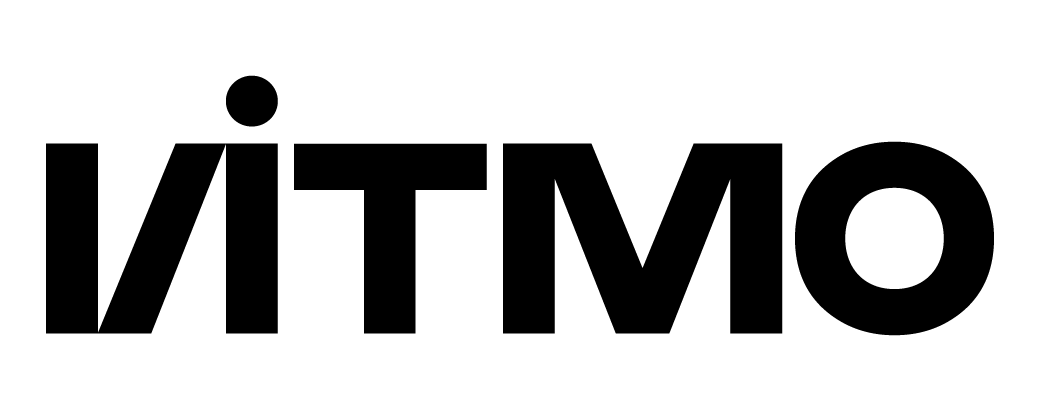
\includegraphics[width=0.3\textwidth]{img/ifmologo.png}\\[0.5cm]
        \textbf{Университет ИТМО}\\[0.3cm]
        Факультет ИТиП\\
        Группа M3232\\[2cm]

        {\Large \textbf{Лабораторная работа №4}}\\[0.5cm]
        {\large Сопряжённые направления и методы Ньютона}\\[0.5cm]
        Дисциплина: Методы оптимизации\\[3cm]

        \begin{flushright}
            Выполнили:\\
            Дегтярев Александр Сергеевич\\
            Надточий Ярослав Вадимофич\\[1cm]
            Проверила: Матвеева М.В.\\
        \end{flushright}

        \vfill
        Санкт-Петербург, 2025
    \end{center}
\end{titlepage}

\tableofcontents
\newpage

%=============================================================================
\section{Постановка задачи}

Исследовать методы второго порядка и квазиньютоновские методы для безусловной минимизации:
\[
    x^* = \arg\min_{x \in \mathbb{R}^n} f(x).
\]

Реализованные методы:
\begin{enumerate}
    \item Метод сопряжённых градиентов для квадратичных функций;
    \item Метод нелинейных сопряжённых градиентов Флетчера--Ривса;
    \item Метод нелинейных сопряжённых градиентов Полака--Рибьера;
    \item Метод Ньютона с использованием разложения Холецкого;
    \item Метод Ньютона с выбором направления;
    \item Метод Powell's Dog Leg;
    \item Квазиньютоновские методы DFP, BFGS и L-BFGS.
\end{enumerate}

Также планировалось сравнение с \texttt{scipy.optimize.minimize(..., method='Newton-CG')}, однако в среде выполнения scipy не был установлен, поэтому данное сравнение не проводилось.

Для каждого метода фиксируются: количество итераций, вычислений функции, градиента и матрицы Гессе (если используется), а также причина остановки.

\subsection*{Модели задач}

\begin{enumerate}
    \item \textbf{Квадратичные функции.} Генератор выпуклых квадратичных функций:
    \[
        f(x) = \frac{1}{2}\langle Ax, x \rangle - \langle b, x \rangle + c, \quad A = A^T \succ 0,
    \]
    с заданной размерностью $n$ и числом обусловленности $\kappa = \text{cond}(A)$. Матрица $A$ строится как $A = Q^T \Lambda Q$, где $Q$~--- случайная ортогональная матрица, $\Lambda$~--- диагональная с собственными значениями от 1 до $\kappa$. Размерности: $n \in \{2, 10, 50, 100\}$, числа обусловленности: $\kappa \in \{1, 10, 100, 1000\}$.

    \item \textbf{Двумерная квадратичная функция} с $n = 2$ и $\kappa = 10$ для визуализации траекторий из 5 различных начальных точек.

    \item \textbf{Тестовые функции:}
    \begin{itemize}
        \item Функция Розенброка: $f(x,y) = (1-x)^2 + 100(y-x^2)^2$, минимум в $(1, 1)$;
        \item Функция Химмельблау: $f(x,y) = (x^2+y-11)^2 + (x+y^2-7)^2$, 4 минимума.
    \end{itemize}
\end{enumerate}

Критерий остановки: $\|\nabla f(x)\| \leq \varepsilon = 10^{-8}$, максимум 3000 итераций (4000 для L-BFGS memory).

%=============================================================================
\section{Теоретические основы}

\subsection{Мотивация: ограничения градиентного спуска}

Градиентный спуск первого порядка использует только информацию о направлении наибыстрейшего убывания $-\nabla f(x)$. Его скорость сходимости на квадратичных задачах ограничена отношением
\[
    \frac{\kappa - 1}{\kappa + 1},
\]
где $\kappa = \lambda_{\max} / \lambda_{\min}$~--- число обусловленности матрицы $A$. При $\kappa = 1000$ фактор сжатия составляет $0.998$, и для уменьшения ошибки в $10^8$ раз потребуется $\sim 9200$ итераций. Методы второго порядка используют информацию о кривизне (гессиан $\nabla^2 f$) и способны достигать квадратичной скорости сходимости, что принципиально ускоряет оптимизацию.

\subsection{Число обусловленности и его влияние}

Число обусловленности $\kappa(A) = \|A\| \cdot \|A^{-1}\|$ характеризует <<вытянутость>> линий уровня функции. При $\kappa = 1$ линии уровня~--- окружности, и все методы сходятся за 1--2 шага. При большом $\kappa$ линии уровня~--- сильно вытянутые эллипсы: градиент указывает не в сторону минимума, а перпендикулярно длинной оси эллипса, что вызывает зигзагообразное поведение у методов первого порядка. Методы, использующие гессиан, масштабируют направление спуска обратной матрицей кривизны, компенсируя вытянутость.

\subsection{Линейный поиск и условия Вольфе}

Многие из реализованных методов используют линейный поиск для определения шага $\alpha_k$. Условия Вольфе обеспечивают достаточное убывание функции (условие Армихо) и ограничивают кривизну:
\[
    f(x_k + \alpha d_k) \leq f(x_k) + c_1 \alpha \nabla f(x_k)^T d_k, \quad
    |\nabla f(x_k + \alpha d_k)^T d_k| \leq c_2 |\nabla f(x_k)^T d_k|,
\]
где $0 < c_1 < c_2 < 1$. Сильные условия Вольфе гарантируют существование допустимого шага для направления спуска и обеспечивают сходимость квазиньютоновских методов.

%=============================================================================
\section{Описание методов}

\subsection{Метод сопряжённых градиентов (квадратичный CG)}

\textbf{Идея.} На квадратичной функции $f(x) = \frac{1}{2}x^TAx - b^Tx + c$ градиентный спуск создаёт зигзаги, потому что каждый следующий градиент ортогонален предыдущему направлению, но не учитывает все предыдущие. Метод CG строит направления $d_0, d_1, \ldots$, которые попарно $A$-сопряжены ($d_i^T A d_j = 0$ при $i \neq j$), что гарантирует: каждый шаг минимизирует функцию в новом подпространстве, не портя результат предыдущих шагов.

\textbf{Алгоритм.} Начальное направление $d_0 = -g_0$. На каждом шаге:
\[
    \alpha_k = -\frac{g_k^T d_k}{d_k^T A d_k}, \quad
    x_{k+1} = x_k + \alpha_k d_k, \quad
    \beta_k = \frac{g_{k+1}^T A d_k}{d_k^T A d_k}, \quad
    d_{k+1} = -g_{k+1} + \beta_k d_k.
\]

\textbf{Свойство.} Гарантированная сходимость за $\leq n$ итераций (точно для квадратичных). Не требует гессиана~--- матрица $A$ используется только через произведение $Ad_k$. Память $O(n)$.

\subsection{Нелинейные методы CG (Флетчер--Ривз, Полак--Рибьер)}

\textbf{Идея.} Обобщение квадратичного CG на произвольные гладкие функции. Поскольку для неквадратичных функций $A$-сопряжённость не определена, используется эвристическая формула для $\beta_k$, основанная только на градиентах.

\textbf{Направление} обновляется как $d_{k+1} = -g_{k+1} + \beta_k d_k$. Два варианта $\beta_k$:
\[
    \beta_k^{\text{FR}} = \frac{\|g_{k+1}\|^2}{\|g_k\|^2}, \qquad
    \beta_k^{\text{PR}} = \frac{g_{k+1}^T(g_{k+1} - g_k)}{\|g_k\|^2}.
\]

\textbf{Различия.} FR сохраняет сопряжённость вдали от минимума, но может <<застревать>> с малым шагом. PR при $\beta_k < 0$ автоматически перезапускается ($\beta_k := 0$), что часто ускоряет сходимость на сильно нелинейных функциях, но увеличивает общее число перезапусков.

\textbf{Шаг} $\alpha_k$ определяется линейным поиском с условиями Вольфе. На квадратичных функциях оба метода совпадают с классическим CG.

\subsection{Метод Ньютона с разложением Холецкого}

\textbf{Идея.} Минимизируем квадратичную модель функции в текущей точке:
\[
    f(x_k + d) \approx f(x_k) + g_k^T d + \frac{1}{2} d^T H_k d,
\]
где $H_k = \nabla^2 f(x_k)$~--- гессиан. Минимум достигается при $H_k d = -g_k$.

\textbf{Почему Холецкий.} Если $H_k$ положительно определена ($H_k \succ 0$), система решается разложением $H_k = LL^T$, что стоит $O(n^3/3)$ операций и численно устойчиво.

\textbf{Сходимость.} Квадратичная: $\|x_{k+1} - x^*\| \leq C \|x_k - x^*\|^2$ вблизи $x^*$. Для квадратичных функций~--- точное решение за 1 итерацию ($H_k = A = \text{const}$).

\textbf{Ограничение.} Если $H_k$ не положительно определена (седловая точка, максимум или вырожденность), разложение Холецкого не существует и метод не может определить направление спуска.

\subsection{Метод Ньютона с выбором направления}

\textbf{Идея.} Модификация метода Ньютона, которая обрабатывает случай, когда $H_k$ не является положительно определённой. Алгоритм:
\begin{enumerate}
    \item Попытаться решить $H_k d = -g_k$ через разложение Холецкого.
    \item Если разложение не удалось~--- использовать направление антиградиента: $d = -g_k$.
    \item Определить шаг $\alpha_k$ линейным поиском с условиями Вольфе.
\end{enumerate}

Линейный поиск обеспечивает гарантированное убывание $f$, даже когда используется антиградиент. Метод комбинирует квадратичную скорость Ньютона вблизи минимума и глобальную сходимость градиентного спуска вдали.

\subsection{Метод области доверия (Powell's Dog Leg)}

\textbf{Идея.} Вместо линейного поиска ограничиваем шаг областью доверия~--- шаром радиуса $\Delta_k$, в пределах которого квадратичная модель <<заслуживает доверия>>:
\[
    \min_{d} \; m_k(d) = f_k + g_k^T d + \frac{1}{2} d^T H_k d, \quad \|d\| \leq \Delta_k.
\]

\textbf{Два крайних случая:}
\begin{itemize}
    \item Если ньютоновский шаг $d^N = -H_k^{-1}g_k$ помещается в область ($\|d^N\| \leq \Delta_k$), используем его~--- максимальная скорость.
    \item Если нет, рассматриваем шаг Коши $d^C = -\frac{g_k^T g_k}{g_k^T H_k g_k} g_k$ (наискорейший спуск с оптимальным шагом по модели).
\end{itemize}

\textbf{Dogleg} аппроксимирует решение кусочно-линейной кривой от начала через $d^C$ к $d^N$, выбирая точку пересечения с границей $\|d\| = \Delta_k$.

\textbf{Адаптация радиуса.} После шага вычисляется отношение $\rho_k = (f(x_k) - f(x_{k+1})) / (m_k(0) - m_k(d_k))$. Если $\rho_k$ близко к 1~--- модель хорошая, $\Delta$ увеличивается. Если $\rho_k$ мало или отрицательно~--- шаг отклоняется, $\Delta$ уменьшается. Это обеспечивает глобальную сходимость без явного линейного поиска.

\subsection{Квазиньютоновские методы: DFP и BFGS}

\textbf{Мотивация.} Методы Ньютона требуют вычисления и хранения гессиана~--- $O(n^2)$ памяти и $O(n^2)$ или $O(n^3)$ операций на каждой итерации (для вычисления и факторизации). Квазиньютоновские методы строят аппроксимацию обратного гессиана $B_k \approx H_k^{-1}$, обновляя её по информации из предыдущих шагов, без явного вычисления $H_k$.

\textbf{Общая схема.} Направление спуска $d_k = -B_k g_k$. После шага обновляем $B_k$ так, чтобы выполнялось секущее условие:
\[
    B_{k+1} y_k = s_k, \quad \text{где } s_k = x_{k+1} - x_k, \; y_k = g_{k+1} - g_k.
\]

\textbf{DFP} (Давидон--Флетчер--Пауэлл)~--- первая квазиньютоновская формула:
\[
    B_{k+1} = B_k - \frac{B_k y_k y_k^T B_k}{y_k^T B_k y_k} + \frac{s_k s_k^T}{y_k^T s_k}.
\]

\textbf{BFGS} (Бройден--Флетчер--Гольдфарб--Шанно)~--- дуальная формула:
\[
    B_{k+1} = \left(I - \frac{s_k y_k^T}{y_k^T s_k}\right) B_k \left(I - \frac{y_k s_k^T}{y_k^T s_k}\right) + \frac{s_k s_k^T}{y_k^T s_k}.
\]

\textbf{Почему BFGS лучше DFP.} BFGS более устойчив к ошибкам линейного поиска и числовым погрешностям: при неточном $\alpha_k$ обновление DFP может сильно исказить $B_k$, тогда как BFGS <<самокорректируется>> за несколько шагов. На практике BFGS рекомендуется как метод по умолчанию.

\textbf{Сходимость.} Суперлинейная: $\|x_{k+1} - x^*\| / \|x_k - x^*\| \to 0$. На квадратичных функциях накапливает точную $H^{-1}$ за $n$ шагов (свойство конечной сходимости).

\textbf{Условие корректности.} Обновление $B_k$ сохраняет положительную определённость при $y_k^T s_k > 0$, что гарантируется условиями Вольфе. Если $y_k^T s_k \leq 0$, обновление пропускается.

\subsection{L-BFGS (ограниченная память)}

\textbf{Проблема.} BFGS хранит матрицу $B_k$ размера $n \times n$~--- при $n = 10^6$ это 8 ТБ в double. L-BFGS решает эту проблему: вместо матрицы хранит последние $m$ пар $(s_i, y_i)$ и вычисляет $B_k g_k$ <<на лету>> за $O(mn)$ операций с помощью алгоритма two-loop recursion.

\textbf{Параметр $m$} (размер памяти, обычно 3--20) определяет компромисс между качеством аппроксимации и расходом памяти. Больше $m$~--- точнее аппроксимация, но дороже итерация. Типичный выбор $m = 10$.

%=============================================================================
\section{Результаты}

\subsection{Квадратичные функции: зависимость от размерности и обусловленности}

\textbf{Зачем этот эксперимент.} Квадратичные функции~--- основной теоретический бенчмарк для методов оптимизации. На них точно известен минимум ($x^* = A^{-1}b$), можно контролировать сложность задачи через $n$ и $\kappa$, и аналитически предсказать поведение каждого метода. Это позволяет проверить корректность реализации: метод Ньютона обязан сойтись за 1 итерацию, CG~--- за $\leq n$.

\textbf{Что ожидаем.} Методы, использующие точный гессиан, не должны зависеть от $\kappa$. Методы первого порядка (нелинейные CG) должны деградировать с ростом $\kappa$. Квазиньютоновские~--- занимать промежуточное положение.

\begin{table}[H]
\centering
\caption{Число итераций на квадратичных функциях ($n=2$)}
\begin{adjustbox}{max width=\textwidth}
\begin{tabular}{lcccc}
\toprule
\textbf{Метод} & $\kappa=1$ & $\kappa=10$ & $\kappa=100$ & $\kappa=1000$ \\
\midrule
Quadratic CG        & 1 & 2  & 2    & 2    \\
Nonlinear CG (FR)   & 1 & 41 & 2426 & $>$3000 \\
Nonlinear CG (PR)   & 1 & 35 & $>$3000 & $>$3000 \\
Newton (Cholesky)   & 1 & 1  & 1    & 1    \\
Newton (direction)  & 1 & 1  & 1    & 1    \\
Dogleg              & 2 & 2  & 1    & 2    \\
DFP                 & 1 & 4  & 3    & 3    \\
BFGS                & 1 & 6  & 3    & 3    \\
L-BFGS              & 1 & 9  & 5    & 13   \\
\bottomrule
\end{tabular}
\end{adjustbox}
\end{table}

\begin{table}[H]
\centering
\caption{Число итераций на квадратичных функциях ($n=10$)}
\begin{adjustbox}{max width=\textwidth}
\begin{tabular}{lcccc}
\toprule
\textbf{Метод} & $\kappa=1$ & $\kappa=10$ & $\kappa=100$ & $\kappa=1000$ \\
\midrule
Quadratic CG        & 1  & 10 & 12   & 14    \\
Nonlinear CG (FR)   & 1  & 99 & $>$3000 & $>$3000 \\
Nonlinear CG (PR)   & 1  & 61 & $>$3000 & $>$3000 \\
Newton (Cholesky)   & 1  & 1  & 1    & 1     \\
Newton (direction)  & 1  & 1  & 1    & 1     \\
Dogleg              & 3  & 3  & 3    & 2     \\
DFP                 & 1  & 20 & $>$3000 & 17    \\
BFGS                & 1  & 19 & 19   & $>$3000 \\
L-BFGS              & 1  & 32 & $>$3000 & $>$3000 \\
\bottomrule
\end{tabular}
\end{adjustbox}
\end{table}

\begin{table}[H]
\centering
\caption{Число итераций на квадратичных функциях ($n=100$)}
\begin{adjustbox}{max width=\textwidth}
\begin{tabular}{lcccc}
\toprule
\textbf{Метод} & $\kappa=1$ & $\kappa=10$ & $\kappa=100$ & $\kappa=1000$ \\
\midrule
Quadratic CG        & 1  & 33  & 90    & 221    \\
Nonlinear CG (FR)   & 1  & $>$3000 & $>$3000 & $>$3000 \\
Nonlinear CG (PR)   & 1  & $>$3000 & $>$3000 & $>$3000 \\
Newton (Cholesky)   & 1  & 1   & 1     & 1      \\
Newton (direction)  & 1  & 1   & 1     & 1      \\
Dogleg              & 4  & 4   & 4     & 4      \\
DFP                 & 1  & $>$3000 & $>$3000 & $>$3000 \\
BFGS                & 1  & $>$3000 & $>$3000 & $>$3000 \\
L-BFGS              & 1  & $>$3000 & $>$3000 & $>$3000 \\
\bottomrule
\end{tabular}
\end{adjustbox}
\end{table}

Методы Ньютона (Cholesky и direction) решают квадратичную задачу за 1 итерацию при любых $n$ и $\kappa$. Квадратичный CG масштабируется линейно по $\kappa$ (теоретически за $\leq n$ шагов). Нелинейные CG и квазиньютоновские методы теряют эффективность при росте $n$ и $\kappa$.

\begin{figure}[H]
\centering
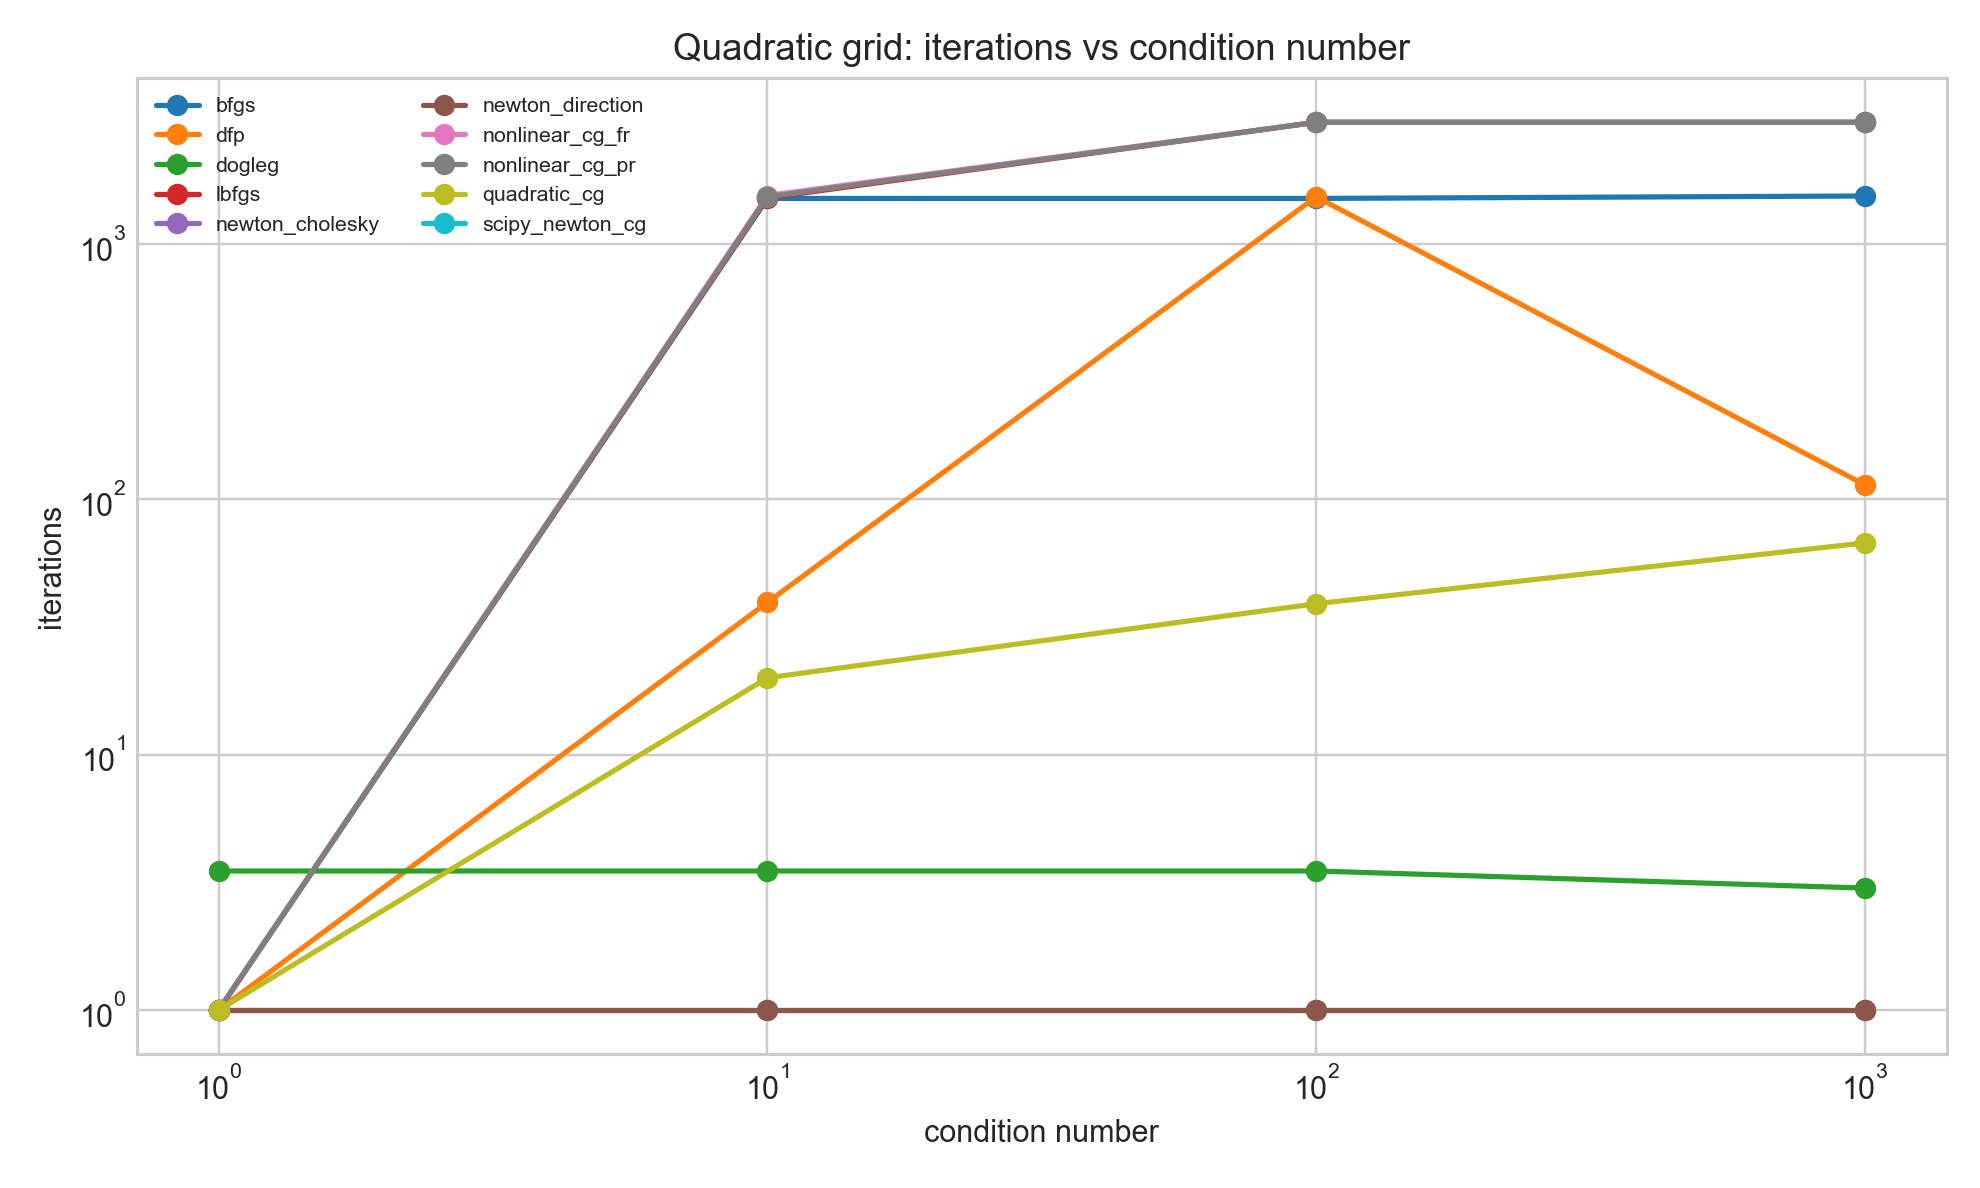
\includegraphics[width=0.85\textwidth]{quadratic_grid/iterations_vs_condition.png}
\caption{Зависимость числа итераций от числа обусловленности}
\end{figure}

\begin{figure}[H]
\centering
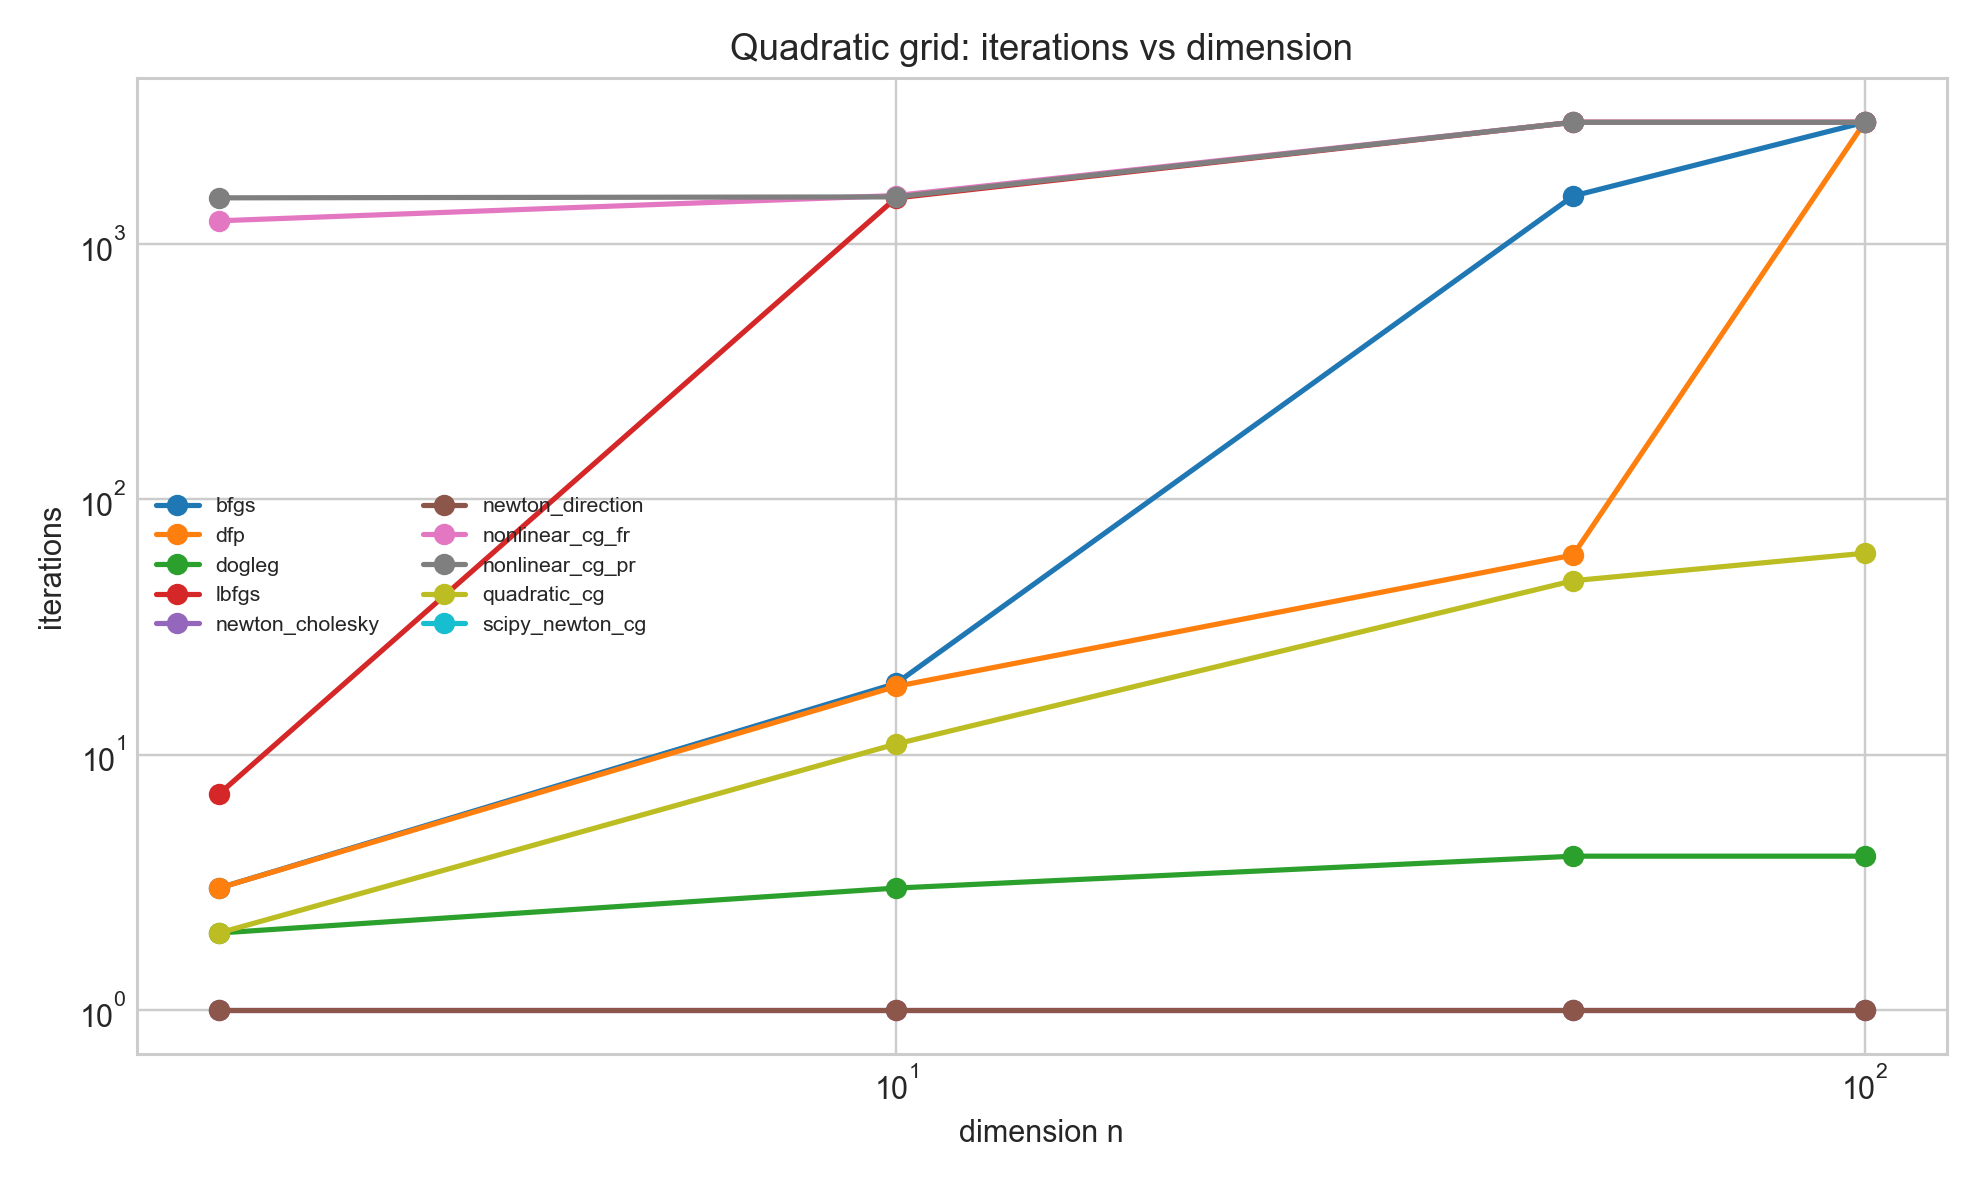
\includegraphics[width=0.85\textwidth]{quadratic_grid/iterations_vs_n.png}
\caption{Зависимость числа итераций от размерности}
\end{figure}

\begin{figure}[H]
\centering
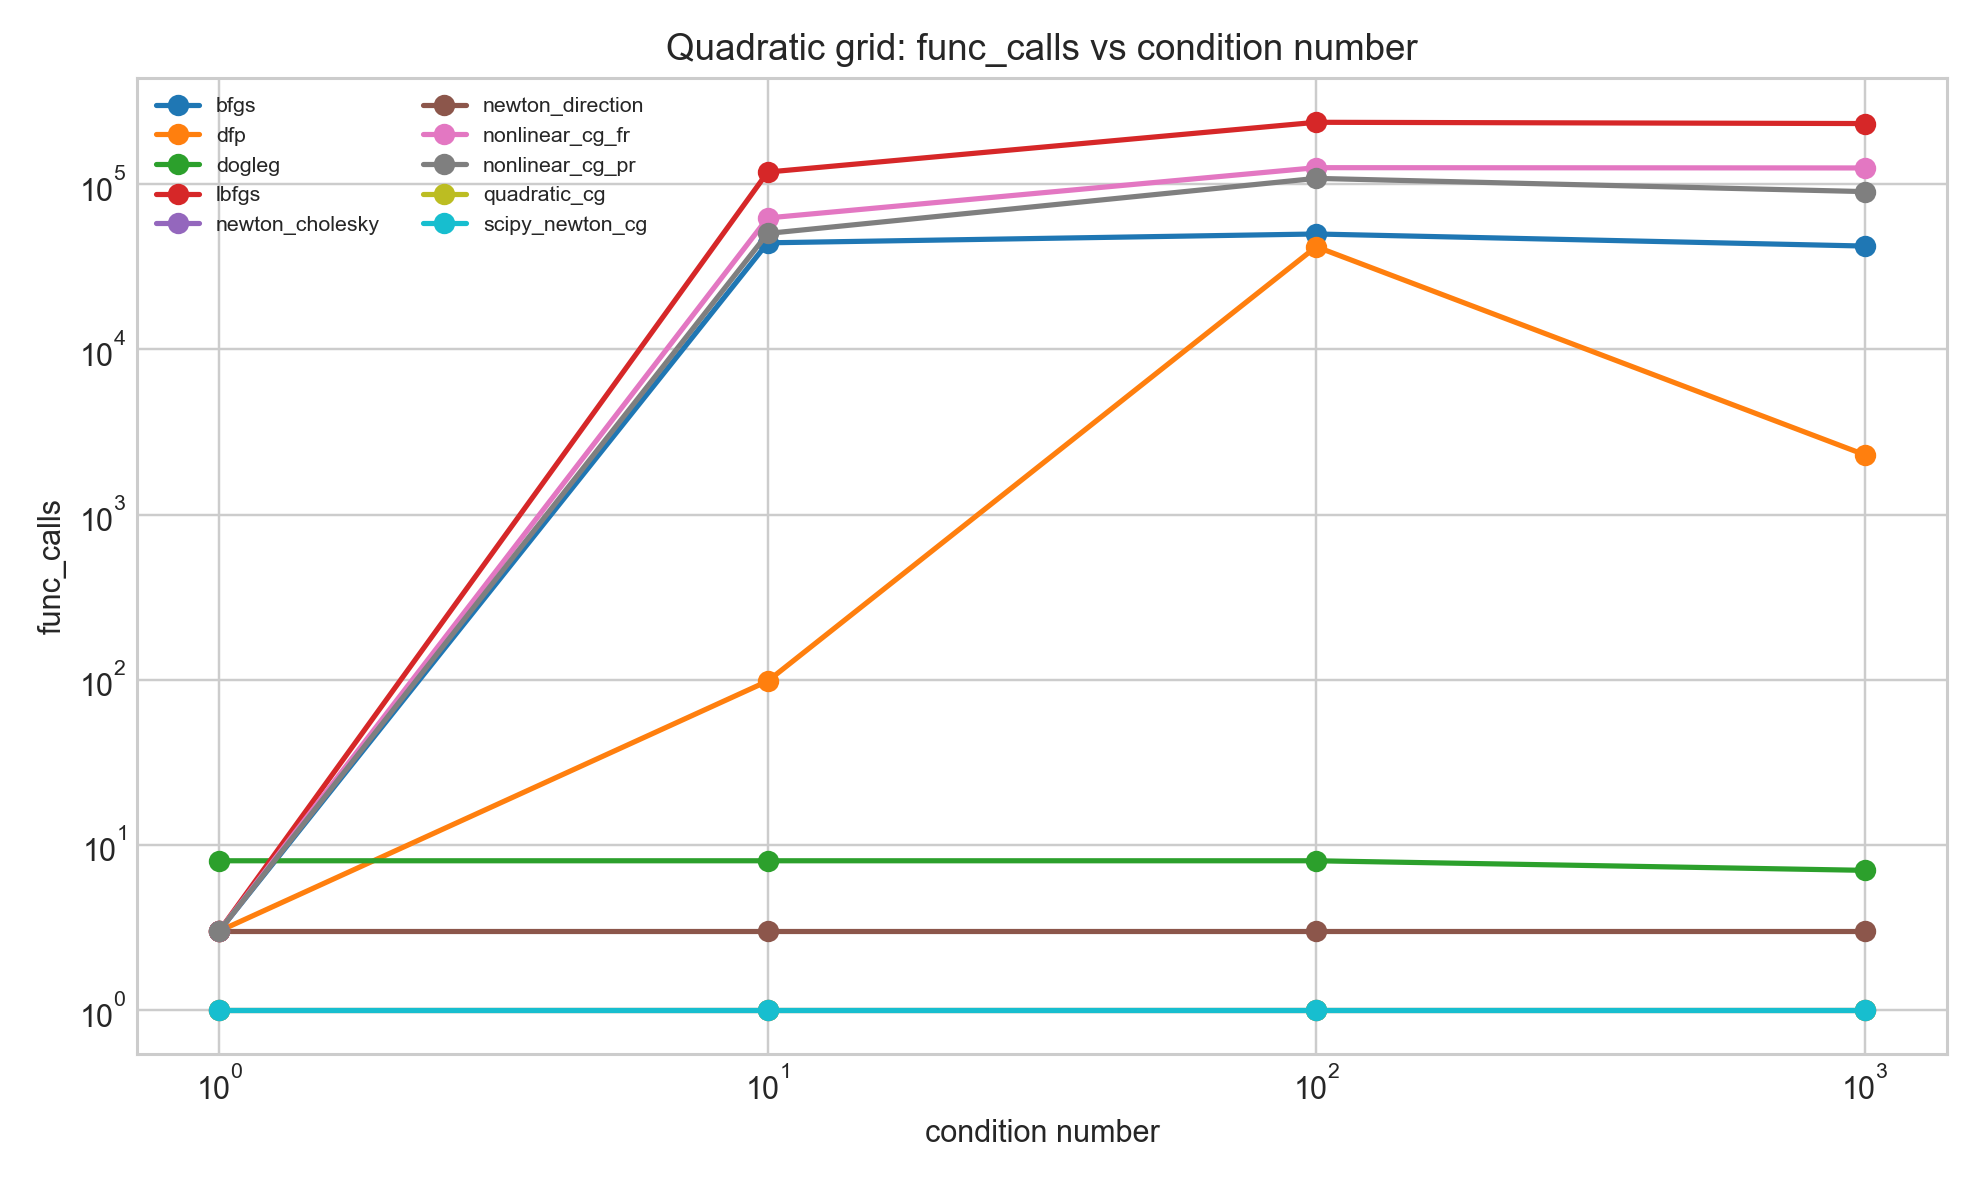
\includegraphics[width=0.85\textwidth]{quadratic_grid/func_calls_vs_condition.png}
\caption{Число вычислений функции от числа обусловленности}
\end{figure}

\begin{figure}[H]
\centering
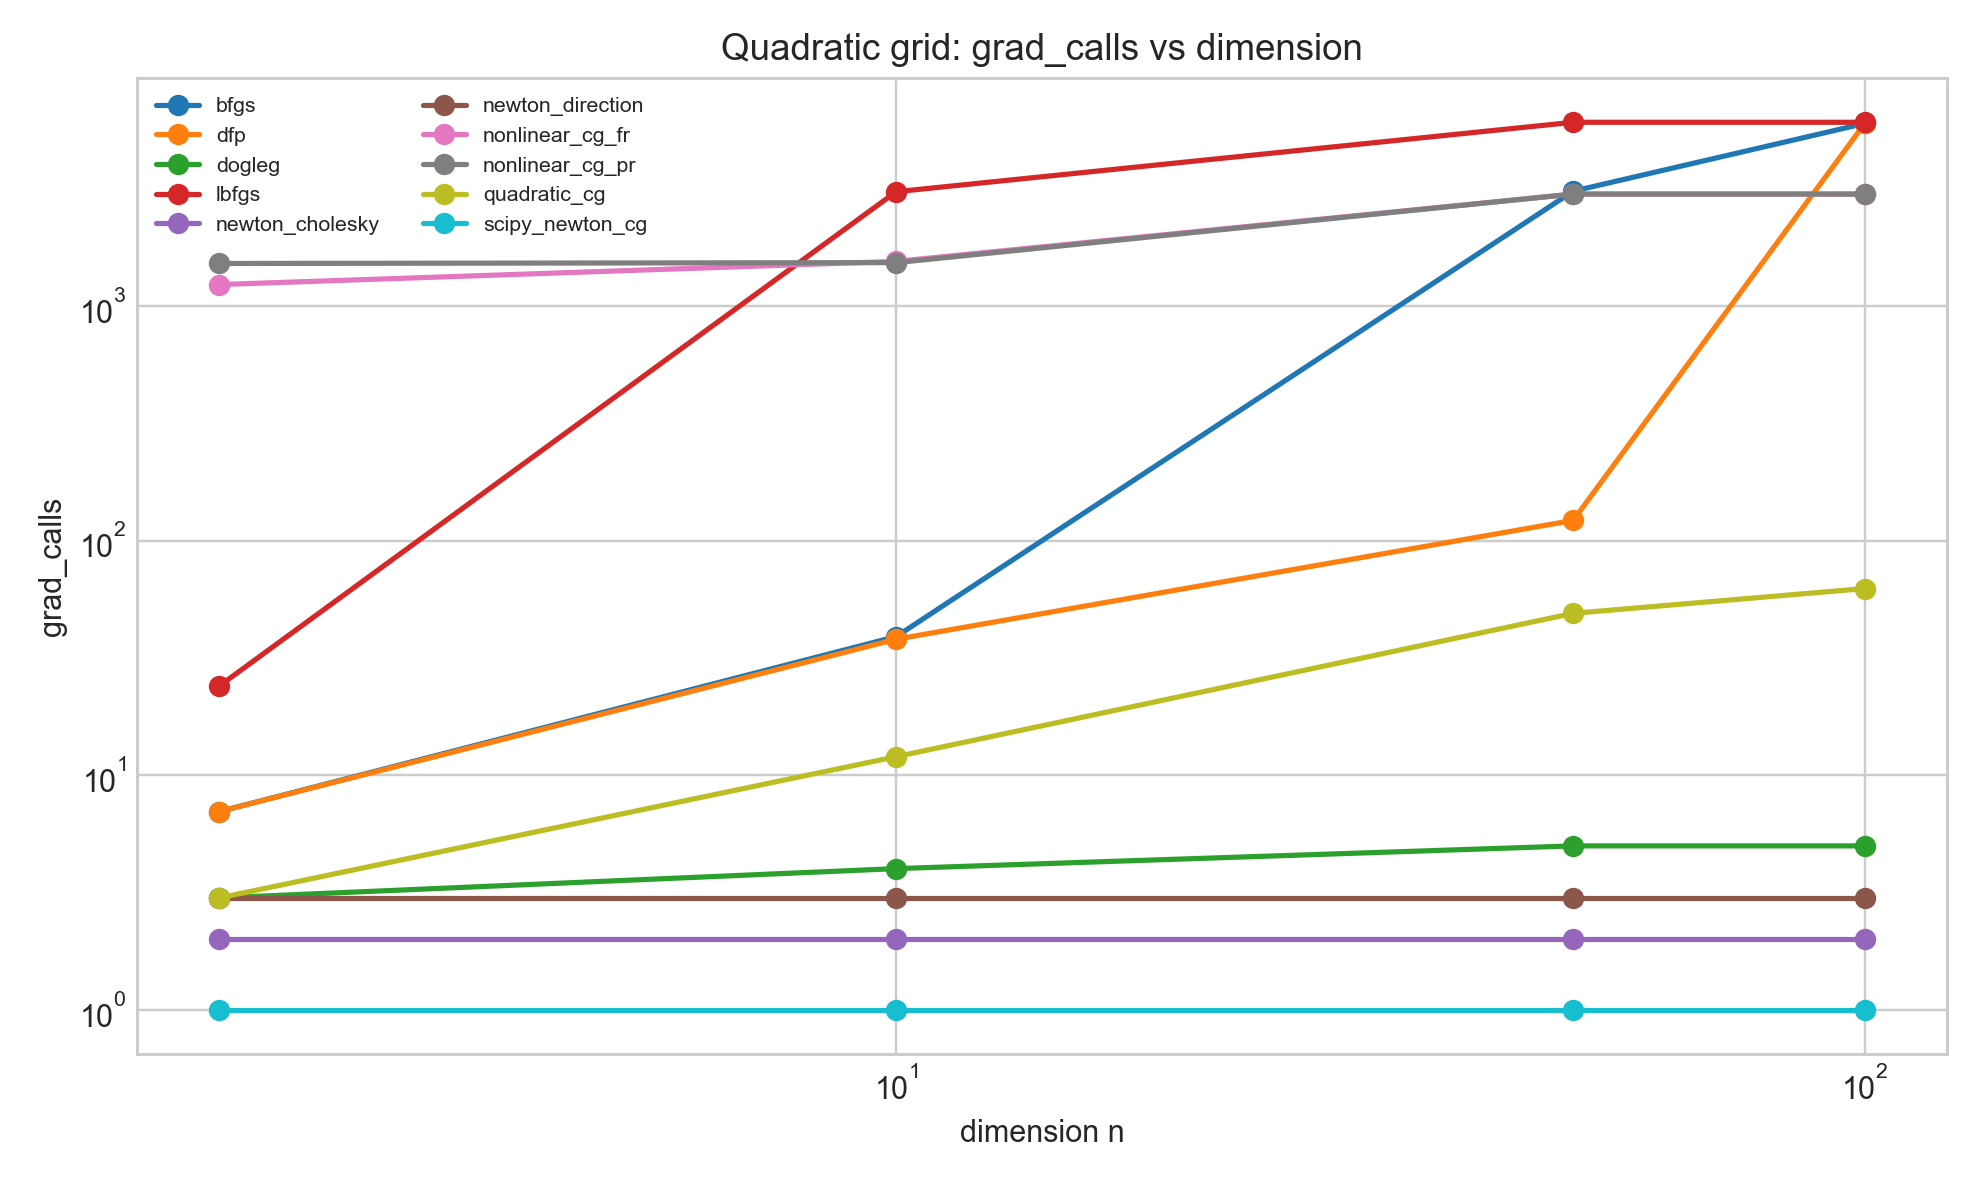
\includegraphics[width=0.85\textwidth]{quadratic_grid/grad_calls_vs_n.png}
\caption{Число вычислений градиента от размерности}
\end{figure}

\subsection{Траектории на 2D квадратичной функции}

Двумерная квадратичная функция с $n = 2$, $\kappa = 10$. Выбрано 5 начальных точек, расположенных на разном расстоянии от минимума и в разных направлениях. Методы Ньютона делают один шаг прямо в минимум. Квазиньютоновские методы постепенно приближаются к квадратичной скорости по мере накопления информации о кривизне. Нелинейные CG демонстрируют зигзагообразные траектории при плохой обусловленности.

\begin{figure}[H]
\centering
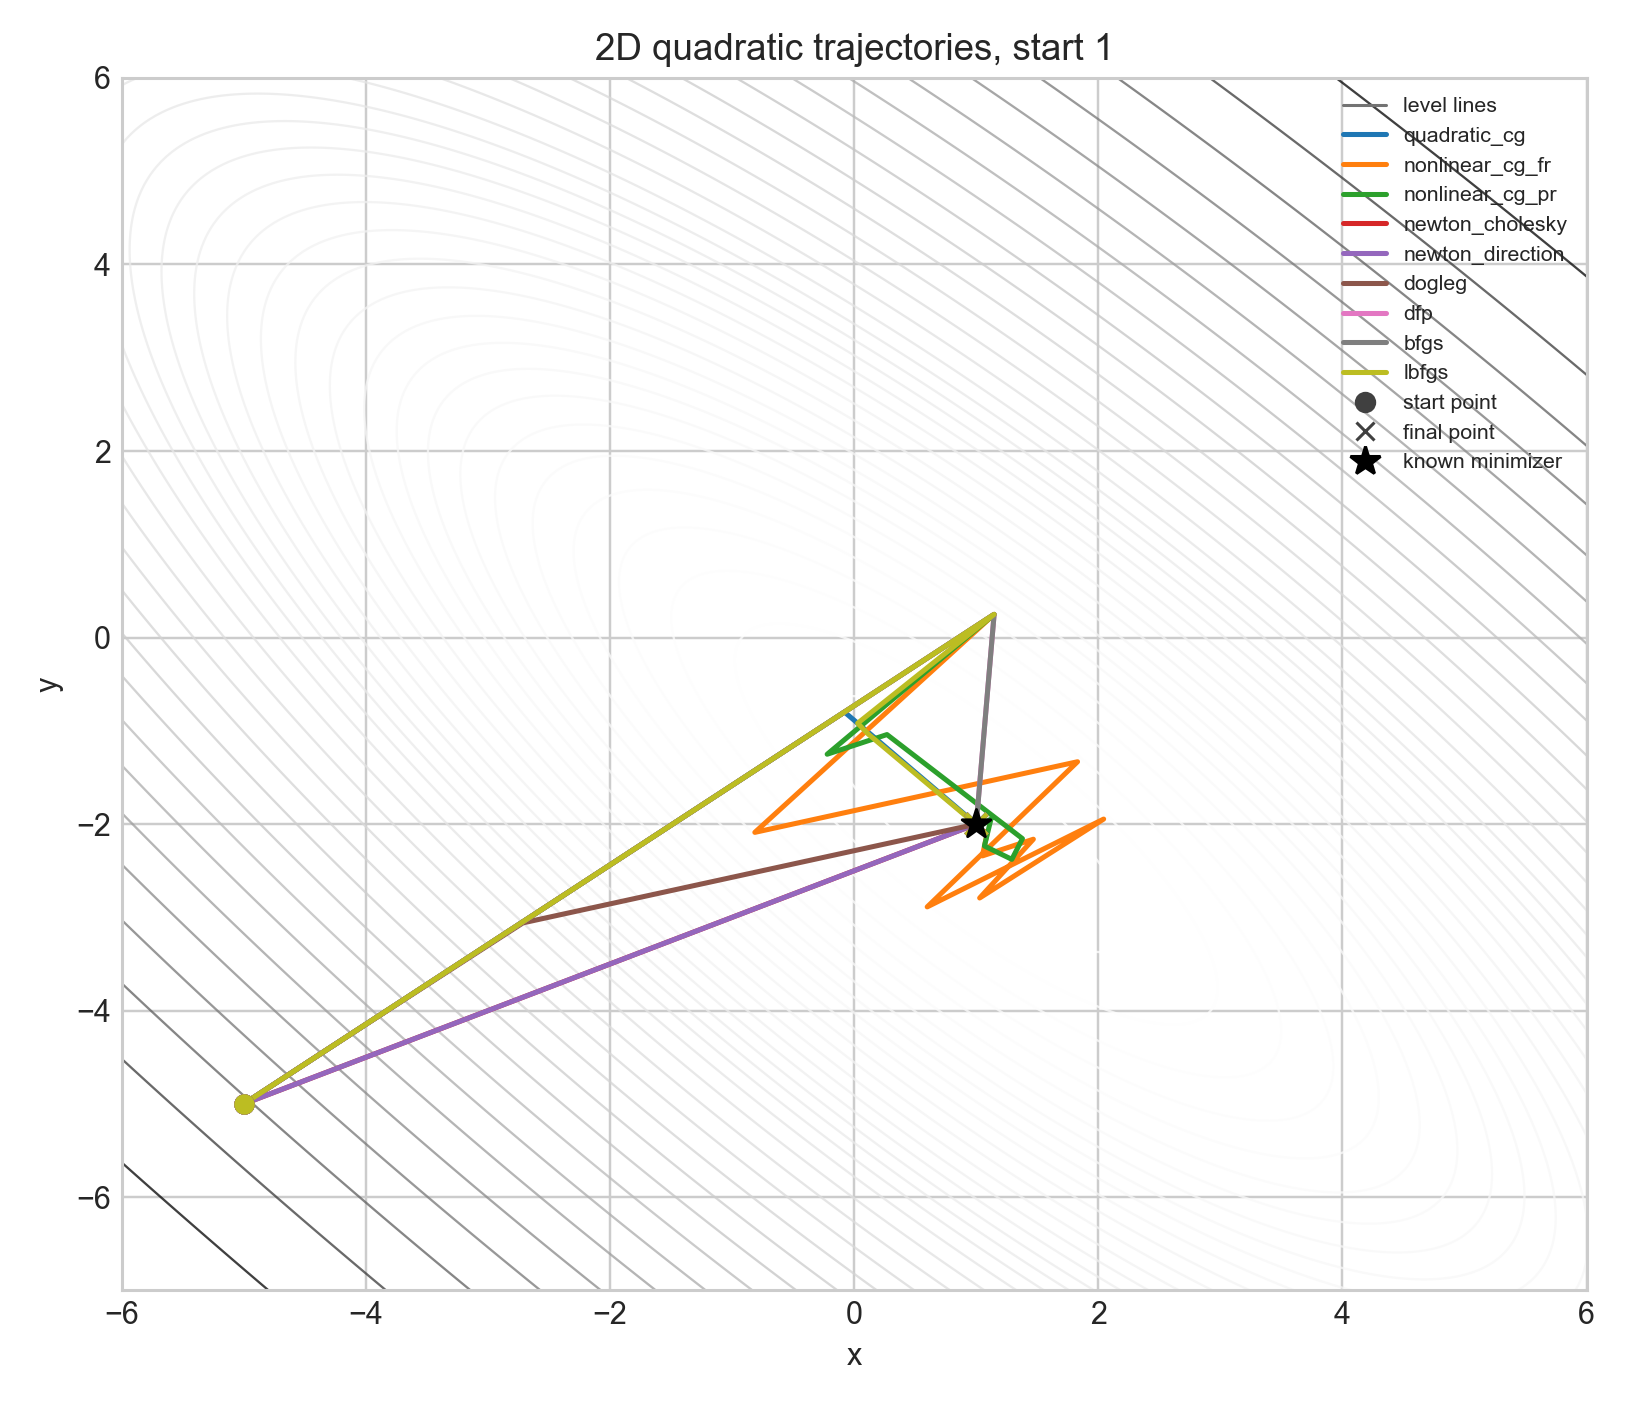
\includegraphics[width=0.85\textwidth]{quadratic_2d_trajectories/start_1.png}
\caption{Траектории оптимизации, начальная точка 1}
\end{figure}

\begin{figure}[H]
\centering
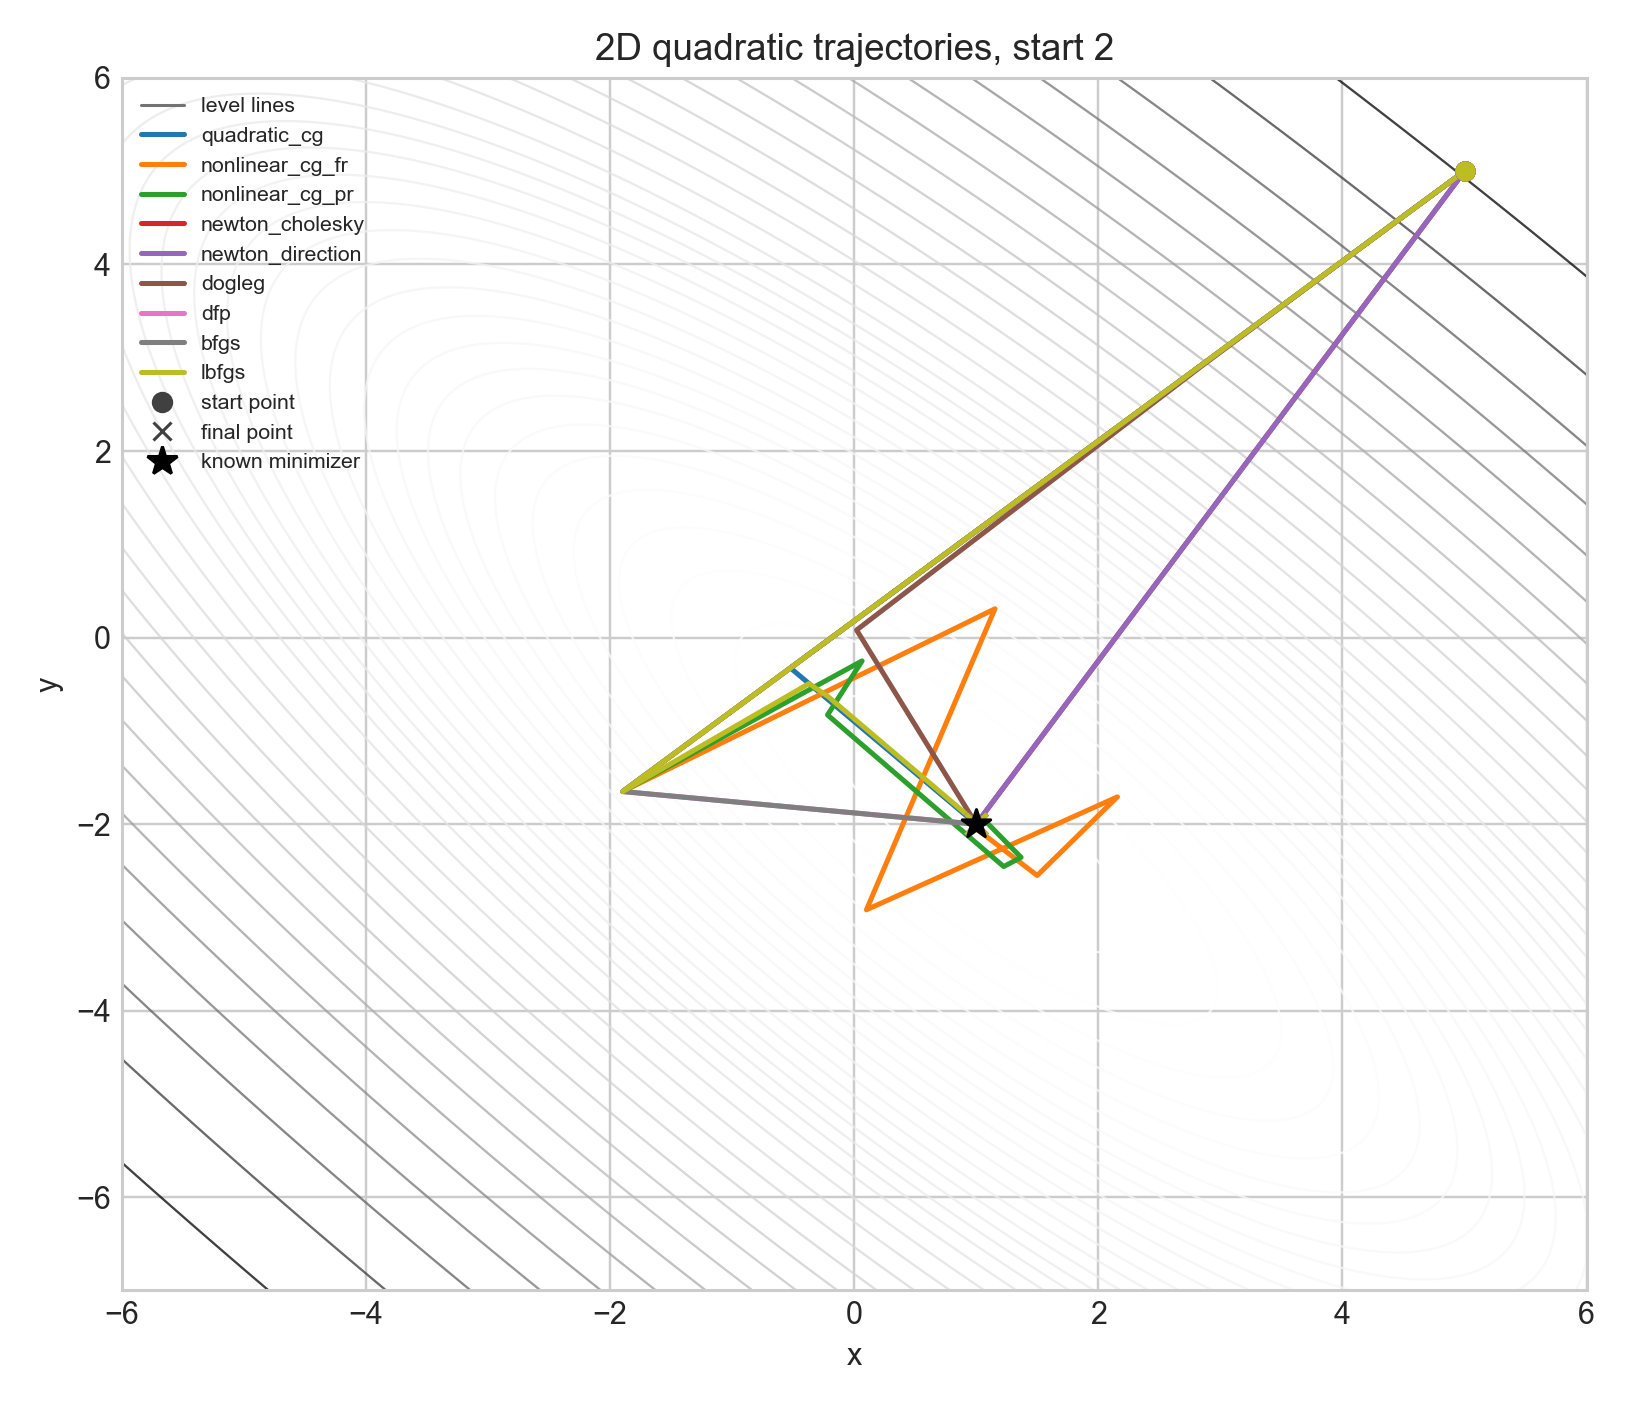
\includegraphics[width=0.85\textwidth]{quadratic_2d_trajectories/start_2.png}
\caption{Траектории оптимизации, начальная точка 2}
\end{figure}

\begin{figure}[H]
\centering
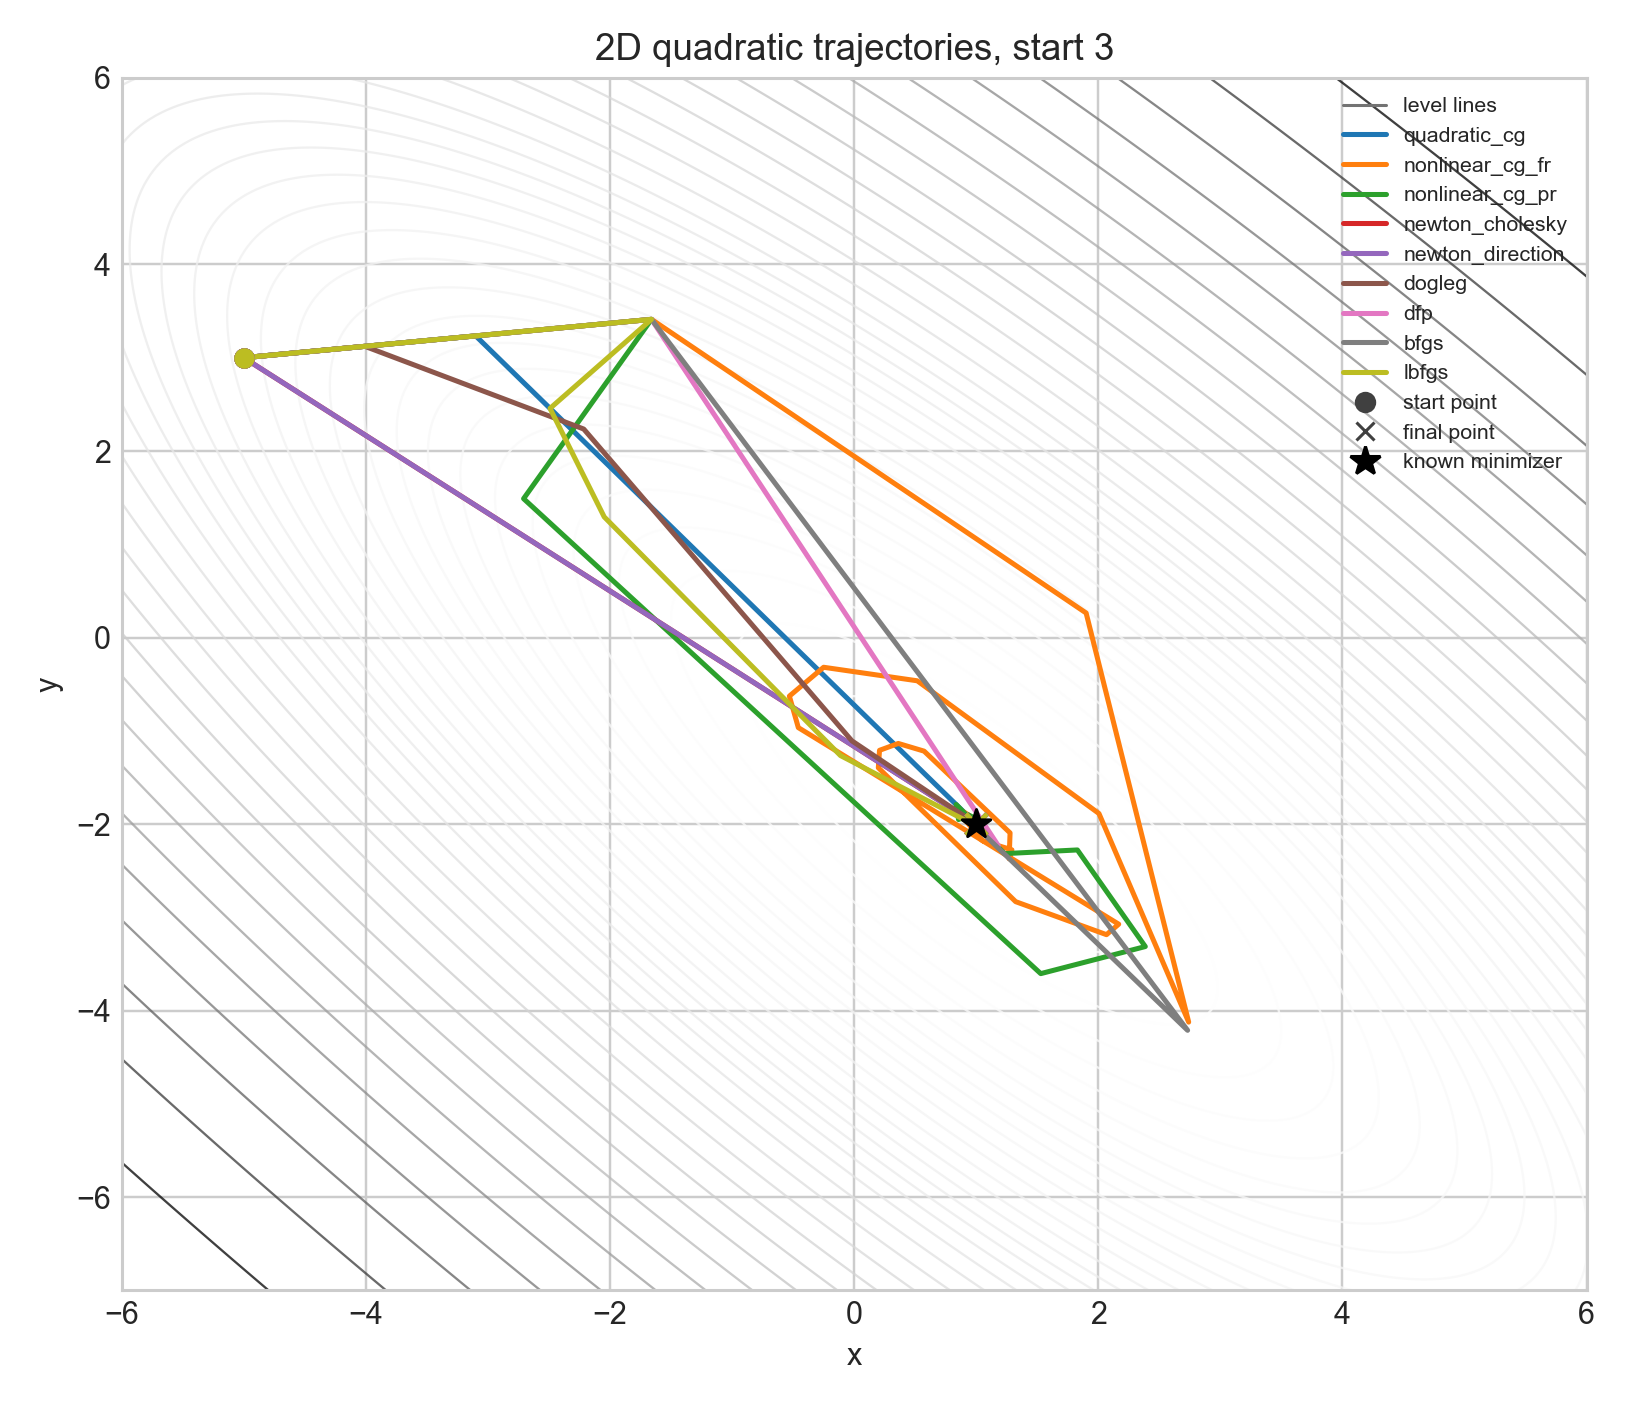
\includegraphics[width=0.85\textwidth]{quadratic_2d_trajectories/start_3.png}
\caption{Траектории оптимизации, начальная точка 3}
\end{figure}

\begin{figure}[H]
\centering
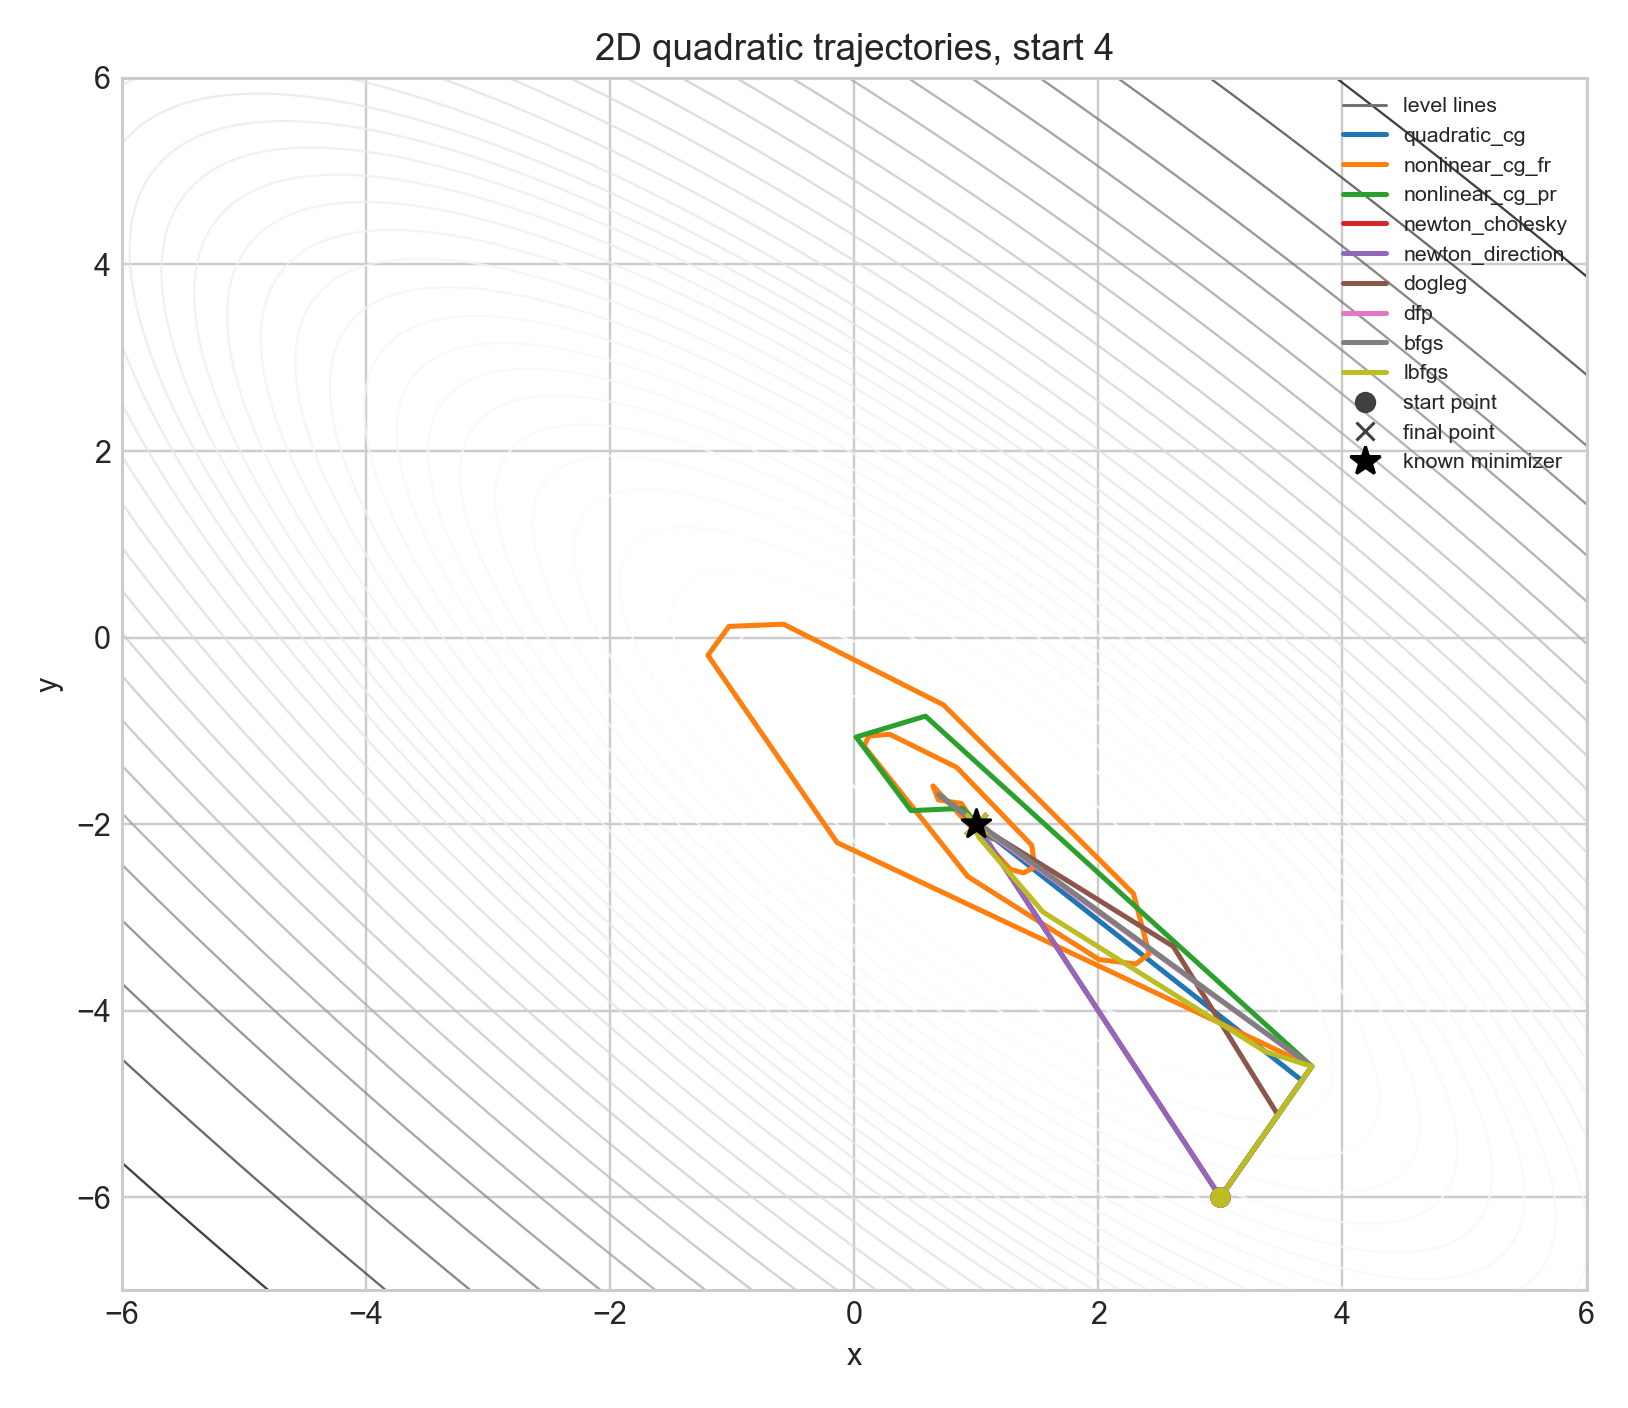
\includegraphics[width=0.85\textwidth]{quadratic_2d_trajectories/start_4.png}
\caption{Траектории оптимизации, начальная точка 4}
\end{figure}

\begin{figure}[H]
\centering
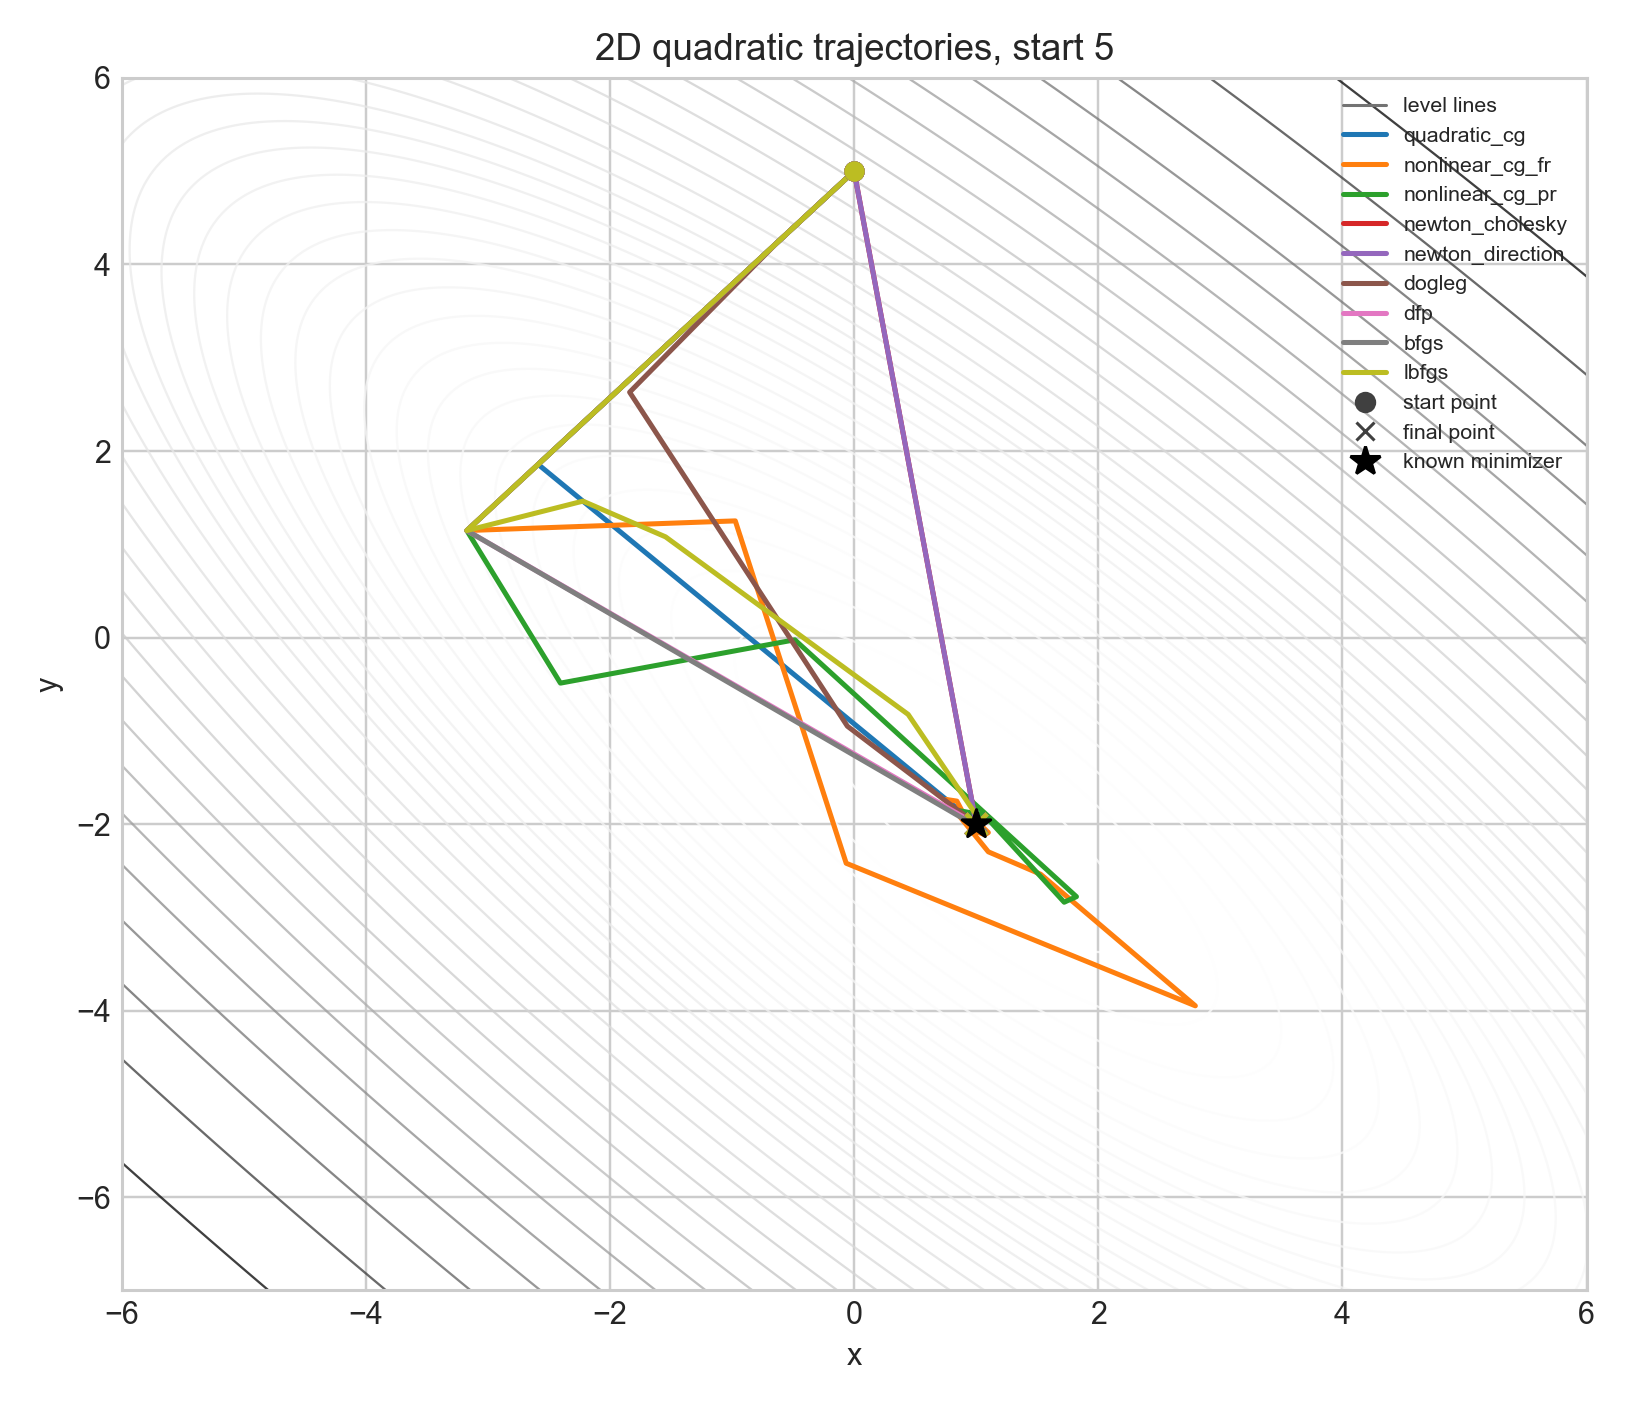
\includegraphics[width=0.85\textwidth]{quadratic_2d_trajectories/start_5.png}
\caption{Траектории оптимизации, начальная точка 5}
\end{figure}

\subsection{Тестовые функции}

\textbf{Зачем этот эксперимент.} Квадратичные функции не отражают трудности реальной оптимизации: нелинейность, несколько локальных минимумов, седловые точки, узкие долины. Тестовые функции Розенброка и Химмельблау~--- классические бенчмарки, демонстрирующие разные типы сложностей. Запуск из нескольких начальных точек позволяет оценить глобальную сходимость и устойчивость к выбору старта.

\subsubsection{Функция Розенброка}

Функция $f(x,y) = (1-x)^2 + 100(y-x^2)^2$ имеет единственный минимум в $(1, 1)$, но оптимизация затруднена узкой параболической долиной: вдоль дна долины функция убывает очень медленно (масштаб $\sim 1$), а поперёк~--- очень быстро (масштаб $\sim 100$). Это создаёт эффективное число обусловленности $\sim 10^3$ вблизи минимума, что критично для методов первого порядка.

\begin{table}[H]
\centering
\caption{Результаты на функции Розенброка, $x_0 = (-1.2, 1)$}
\begin{adjustbox}{max width=\textwidth}
\begin{tabular}{lrrrrcr}
\toprule
\textbf{Метод} & \textbf{Итер.} & \textbf{$f$-выч.} & \textbf{$\nabla f$-выч.} & \textbf{$H$-выч.} & \textbf{Сходимость} & $f(x^*)$ \\
\midrule
CG (FR)            & 226  & 2979  & 227   & 0  & Да  & $1.9 \cdot 10^{-19}$ \\
CG (PR)            & 1523 & 16703 & 1524  & 0  & Да  & $2.5 \cdot 10^{-18}$ \\
Newton (Cholesky)  & 6    & 1     & 7     & 6  & Да  & $3.4 \cdot 10^{-20}$ \\
Newton (direction) & 21   & 48    & 44    & 21 & Да  & $7.7 \cdot 10^{-24}$ \\
Dogleg             & 24   & 49    & 25    & 24 & Да  & $8.6 \cdot 10^{-22}$ \\
DFP                & 50   & 120   & 101   & 0  & Да  & $5.4 \cdot 10^{-21}$ \\
BFGS               & 35   & 90    & 71    & 0  & Да  & $4.3 \cdot 10^{-21}$ \\
L-BFGS             & 35   & 100   & 119   & 0  & Да  & $4.7 \cdot 10^{-22}$ \\
\bottomrule
\end{tabular}
\end{adjustbox}
\end{table}

\begin{table}[H]
\centering
\caption{Результаты на функции Розенброка, $x_0 = (0, 0)$}
\begin{adjustbox}{max width=\textwidth}
\begin{tabular}{lrrrrcr}
\toprule
\textbf{Метод} & \textbf{Итер.} & \textbf{$f$-выч.} & \textbf{$\nabla f$-выч.} & \textbf{$H$-выч.} & \textbf{Сходимость} & $f(x^*)$ \\
\midrule
CG (FR)            & 216  & 2288  & 217   & 0  & Да  & $3.0 \cdot 10^{-18}$ \\
CG (PR)            & 1063 & 11639 & 1064  & 0  & Да  & $1.0 \cdot 10^{-17}$ \\
Newton (Cholesky)  & 2    & 1     & 3     & 2  & Да  & $4.9 \cdot 10^{-30}$ \\
Newton (direction) & 14   & 34    & 31    & 14 & Да  & $1.6 \cdot 10^{-21}$ \\
Dogleg             & 15   & 31    & 16    & 15 & Да  & $9.7 \cdot 10^{-28}$ \\
DFP                & 29   & 66    & 59    & 0  & Да  & $7.0 \cdot 10^{-20}$ \\
BFGS               & 27   & 67    & 55    & 0  & Да  & $3.2 \cdot 10^{-23}$ \\
L-BFGS             & 22   & 53    & 69    & 0  & Да  & $1.2 \cdot 10^{-26}$ \\
\bottomrule
\end{tabular}
\end{adjustbox}
\end{table}

\begin{table}[H]
\centering
\caption{Результаты на функции Розенброка, $x_0 = (2, 2)$}
\begin{adjustbox}{max width=\textwidth}
\begin{tabular}{lrrrrcr}
\toprule
\textbf{Метод} & \textbf{Итер.} & \textbf{$f$-выч.} & \textbf{$\nabla f$-выч.} & \textbf{$H$-выч.} & \textbf{Сходимость} & $f(x^*)$ \\
\midrule
CG (FR)            & 134  & 1337  & 135    & 0  & Да  & $8.2 \cdot 10^{-18}$ \\
CG (PR)            & 1610 & 17744 & 1611   & 0  & Да  & $1.1 \cdot 10^{-17}$ \\
Newton (Cholesky)  & 5    & 1     & 6      & 5  & Да  & $8.3 \cdot 10^{-30}$ \\
Newton (direction) & 15   & 36    & 33     & 15 & Да  & $2.0 \cdot 10^{-21}$ \\
Dogleg             & 16   & 33    & 17     & 16 & Да  & $5.7 \cdot 10^{-23}$ \\
DFP                & 8000 & 16072 & 16001  & 0  & \textbf{Нет} & $3.0 \cdot 10^{-3}$ \\
BFGS               & 48   & 127   & 97     & 0  & Да  & $4.6 \cdot 10^{-20}$ \\
L-BFGS             & 46   & 114   & 144    & 0  & Да  & $1.7 \cdot 10^{-22}$ \\
\bottomrule
\end{tabular}
\end{adjustbox}
\end{table}

Newton-Cholesky показывает наилучшие результаты: 2--6 итераций, 1 вычисление функции. DFP не сходится из точки $(2, 2)$ за 8000 итераций (357 пропущенных обновлений матрицы). BFGS и L-BFGS стабильно сходятся из всех точек за 22--48 итераций. CG (PR) значительно медленнее FR из-за частых перезапусков.

\begin{figure}[H]
\centering

\includegraphics[width=0.85\textwidth]{test_functions/rosenbrock/start_1.png}
\caption{Траектории на функции Розенброка, $x_0 = (-1.2, 1)$}
\end{figure}

\begin{figure}[H]
\centering

\includegraphics[width=0.85\textwidth]{test_functions/rosenbrock/start_2.png}
\caption{Траектории на функции Розенброка, $x_0 = (0, 0)$}
\end{figure}

\begin{figure}[H]
\centering

\includegraphics[width=0.85\textwidth]{test_functions/rosenbrock/start_3.png}
\caption{Траектории на функции Розенброка, $x_0 = (2, 2)$}
\end{figure}

\subsubsection{Функция Химмельблау}

Функция $f(x,y) = (x^2+y-11)^2 + (x+y^2-7)^2$ имеет 4 глобальных минимума: $(3, 2)$, $(-2.81, 3.13)$, $(-3.78, -3.28)$, $(3.58, -1.85)$, а также седловую точку вблизи начала координат. Точка $(0, 0)$ интересна тем, что гессиан в ней не является положительно определённым ($f(0,0) = 170$, это не минимум), что позволяет протестировать устойчивость методов к некорректному гессиану.

\begin{table}[H]
\centering
\caption{Результаты на функции Химмельблау, $x_0 = (0, 0)$}
\begin{adjustbox}{max width=\textwidth}
\begin{tabular}{lrrrrll}
\toprule
\textbf{Метод} & \textbf{Итер.} & \textbf{$f$-выч.} & \textbf{$\nabla f$} & \textbf{$H$} & \textbf{Сход.} & \textbf{Найденный мин.} \\
\midrule
CG (FR)            & 442  & 4387 & 443  & 0  & Да  & $(3,\;2)$ \\
CG (PR)            & 32   & 250  & 33   & 0  & Да  & $(3,\;2)$ \\
Newton (Cholesky)  & ---  & ---  & ---  & 1  & \textbf{Нет} & гессиан не PD \\
Newton (direction) & 7    & 23   & 16   & 7  & Да  & $(3,\;2)$ \\
Dogleg             & 9    & 19   & 10   & 9  & Да  & $(3,\;2)$ \\
DFP                & 11   & 32   & 23   & 0  & Да  & $(3,\;2)$ \\
BFGS               & 10   & 32   & 21   & 0  & Да  & $(3,\;2)$ \\
L-BFGS             & 11   & 30   & 34   & 0  & Да  & $(3,\;2)$ \\
\bottomrule
\end{tabular}
\end{adjustbox}
\end{table}

\begin{table}[H]
\centering
\caption{Результаты на функции Химмельблау, остальные стартовые точки}
\begin{adjustbox}{max width=\textwidth}
\begin{tabular}{llrrrcl}
\toprule
\textbf{Метод} & $x_0$ & \textbf{Итер.} & \textbf{$f$-выч.} & \textbf{$\nabla f$} & \textbf{Сход.} & \textbf{Найденный мин.} \\
\midrule
Newton (Cholesky) & $(-3,\;3)$   & 4 & 1  & 5  & Да & $(-2.81,\;3.13)$ \\
Newton (direction) & $(-3,\;3)$  & 4 & 9  & 9  & Да & $(-2.81,\;3.13)$ \\
BFGS              & $(-3,\;3)$   & 6 & 24 & 13 & Да & $(-2.81,\;3.13)$ \\
L-BFGS            & $(-3,\;3)$   & 5 & 17 & 16 & Да & $(-2.81,\;3.13)$ \\
\midrule
Newton (Cholesky) & $(3,\;-2)$   & 5 & 1  & 6  & Да & $(3.58,\;-1.85)$ \\
BFGS              & $(3,\;-2)$   & 9 & 29 & 19 & Да & $(3.58,\;-1.85)$ \\
L-BFGS            & $(3,\;-2)$   & 8 & 23 & 25 & Да & $(3.58,\;-1.85)$ \\
\midrule
Newton (Cholesky) & $(-4,\;-4)$  & 5 & 1  & 6  & Да & $(-3.78,\;-3.28)$ \\
BFGS              & $(-4,\;-4)$  & 9 & 31 & 19 & Да & $(-3.78,\;-3.28)$ \\
L-BFGS            & $(-4,\;-4)$  & 8 & 23 & 25 & Да & $(-3.78,\;-3.28)$ \\
\bottomrule
\end{tabular}
\end{adjustbox}
\end{table}

Все методы находят один из 4 минимумов функции Химмельблау в зависимости от начальной точки. Newton-Cholesky не может стартовать из $(0, 0)$, так как гессиан в этой точке не является положительно определённым. Метод Ньютона с выбором направления (Newton-direction) успешно справляется с этой ситуацией, переключаясь на антиградиент с линейным поиском.

\begin{figure}[H]
\centering

\includegraphics[width=0.85\textwidth]{test_functions/himmelblau/start_1.png}
\caption{Траектории на функции Химмельблау, $x_0 = (0, 0)$}
\end{figure}

\begin{figure}[H]
\centering

\includegraphics[width=0.85\textwidth]{test_functions/himmelblau/start_2.png}
\caption{Траектории на функции Химмельблау, $x_0 = (-3, 3)$}
\end{figure}

\begin{figure}[H]
\centering

\includegraphics[width=0.85\textwidth]{test_functions/himmelblau/start_3.png}
\caption{Траектории на функции Химмельблау, $x_0 = (3, -2)$}
\end{figure}

\begin{figure}[H]
\centering

\includegraphics[width=0.85\textwidth]{test_functions/himmelblau/start_4.png}
\caption{Траектории на функции Химмельблау, $x_0 = (-4, -4)$}
\end{figure}

\subsection{Влияние размера памяти L-BFGS}

\textbf{Зачем этот эксперимент.} Параметр памяти $m$ в L-BFGS~--- ключевой компромисс: при $m = n$ метод эквивалентен полному BFGS, при $m = 1$~--- близок к градиентному спуску. Задание требует исследовать, как $m$ влияет на сходимость хотя бы на одной серии задач.

Исследовано влияние параметра памяти $m \in \{3, 5, 10, 20\}$ на квадратичной задаче размерности $n=100$ с $\kappa=1000$. Все конфигурации достигли лимита в 4000 итераций, не сойдясь. Однако при этом значение целевой функции практически одинаково ($f \approx -7751.27$), что говорит о медленной сходимости в последних итерациях.

\begin{table}[H]
\centering
\caption{L-BFGS: влияние размера памяти ($n=100$, $\kappa=1000$)}
\begin{tabular}{ccccc}
\toprule
\textbf{Память $m$} & \textbf{Итер.} & \textbf{$f$-вызовы} & \textbf{$\nabla f$-вызовы} & $\|\nabla f\|$ \\
\midrule
3  & 4000 & 316\,284 & 8293 & $1.60 \cdot 10^{-5}$ \\
5  & 4000 & 313\,436 & 8276 & $1.73 \cdot 10^{-5}$ \\
10 & 4000 & 307\,635 & 8266 & $1.08 \cdot 10^{-5}$ \\
20 & 4000 & 320\,003 & 8268 & $1.13 \cdot 10^{-5}$ \\
\bottomrule
\end{tabular}
\end{table}

Увеличение памяти $m$ не даёт значительного преимущества на этой задаче: все варианты близки к решению, но не достигают порога сходимости $\|\nabla f\| \leq 10^{-8}$.

\begin{figure}[H]
\centering
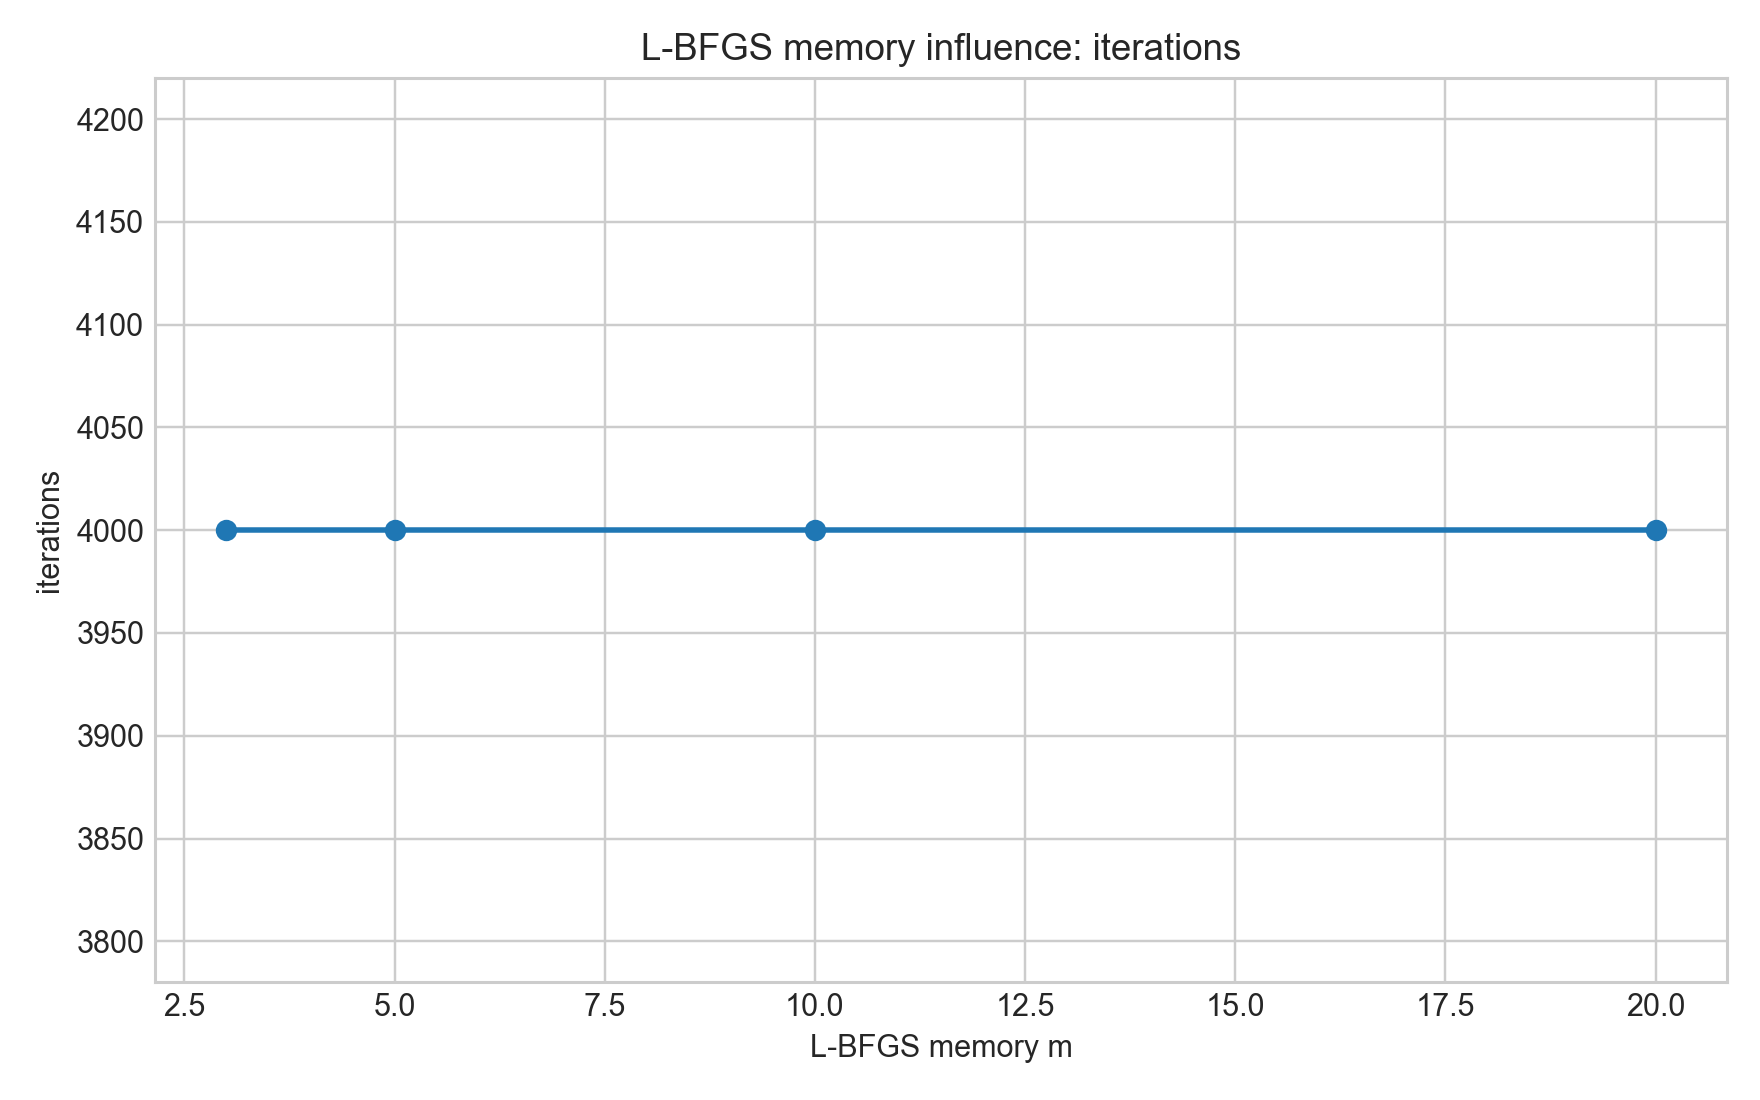
\includegraphics[width=0.85\textwidth]{lbfgs_memory/iterations.png}
\caption{L-BFGS: итерации при разном размере памяти}
\end{figure}

\begin{figure}[H]
\centering
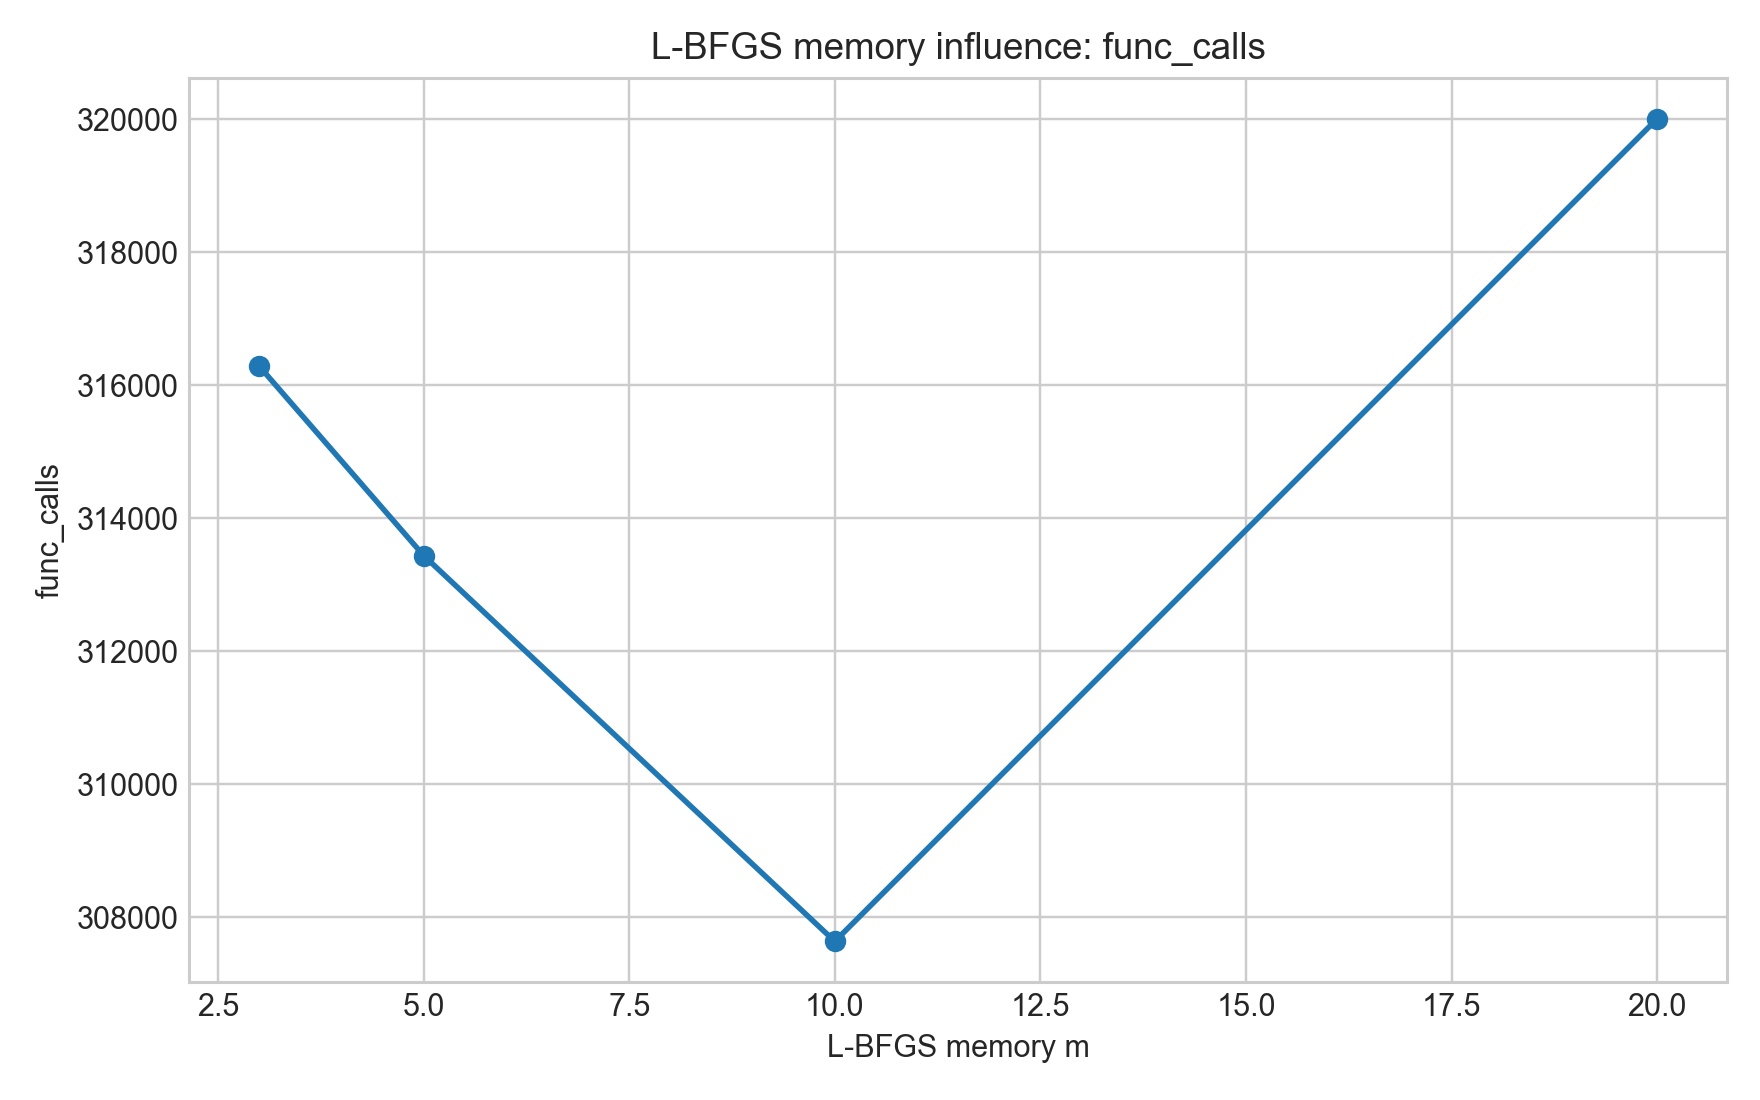
\includegraphics[width=0.85\textwidth]{lbfgs_memory/func_calls.png}
\caption{L-BFGS: вычисления функции при разном размере памяти}
\end{figure}

%=============================================================================
\section{Сравнение методов}

\begin{table}[H]
\centering
\caption{Сравнительная характеристика методов}
\begin{adjustbox}{max width=\textwidth}
\begin{tabular}{lcccl}
\toprule
\textbf{Метод} & \textbf{Гессиан} & \textbf{Память} & \textbf{Скорость сход.} & \textbf{Особенности} \\
\midrule
Quadratic CG & нет & $O(n)$ & $\leq n$ шагов & только квадратичные \\
CG (FR/PR) & нет & $O(n)$ & линейная & перезапуски, чувствителен к $\kappa$ \\
Newton (Cholesky) & да & $O(n^2)$ & квадратичная & требует PD гессиан \\
Newton (direction) & да & $O(n^2)$ & квадратичная & робастнее Cholesky \\
Dogleg & да & $O(n^2)$ & квадратичная & глобальная сходимость \\
DFP & нет & $O(n^2)$ & суперлинейная & менее стабилен, чем BFGS \\
BFGS & нет & $O(n^2)$ & суперлинейная & наиболее надёжный \\
L-BFGS & нет & $O(mn)$ & суперлинейная & для больших $n$ \\
\bottomrule
\end{tabular}
\end{adjustbox}
\end{table}

%=============================================================================
\section{Выводы}

\subsection*{Влияние числа обусловленности}

Число обусловленности $\kappa$ по-разному влияет на разные классы методов:

\begin{itemize}
    \item \textbf{Методы Ньютона} (Cholesky, direction, dogleg) \textit{нечувствительны} к $\kappa$: 1 итерация на квадратичных задачах при любом $\kappa$ и $n$. Используя точную информацию о кривизне (гессиан), они компенсируют плохую обусловленность.

    \item \textbf{Квадратичный CG} линейно зависит от $\kappa$: при $n=100$ число итераций растёт от 1 ($\kappa=1$) до 221 ($\kappa=1000$), оставаясь $\leq n$.

    \item \textbf{Нелинейные CG (FR/PR)} крайне чувствительны: уже при $\kappa=10$, $n=10$ FR требует 99 итераций, а при $\kappa \geq 100$ и $n > 2$ оба метода не сходятся за 3000 итераций. Зигзагообразные траектории на плохо обусловленных задачах приводят к медленной сходимости.

    \item \textbf{Квазиньютоновские методы} (DFP, BFGS, L-BFGS) занимают промежуточное положение. На малых $n$ ($\leq 10$) и умеренных $\kappa$ ($\leq 100$) сходятся за 3--20 итераций. При больших $n$ ($\geq 50$) и $\kappa \geq 10$ не успевают накопить достаточно кривизной информации за 3000 итераций.
\end{itemize}

\subsection*{Требование положительной определённости гессиана}

\begin{itemize}
    \item \textbf{Newton-Cholesky} строго требует PD гессиан. При нарушении (точка $(0,0)$ на Химмельблау) метод не может выполнить даже одну итерацию, т.к. разложение Холецкого не существует.

    \item \textbf{Newton-direction} обходит проблему: при неудачном разложении Холецкого переключается на направление антиградиента с линейным поиском (Вольфе). Это обеспечивает глобальную сходимость (7 итераций из $(0,0)$ на Химмельблау).

    \item \textbf{Dogleg} также требует PD гессиан для построения ньютоновского шага, но механизм области доверия и шаг Коши обеспечивают устойчивость. На Химмельблау из $(0,0)$ догleg сходится за 9 итераций.

    \item \textbf{Квазиньютоновские методы} (DFP, BFGS, L-BFGS) не используют гессиан напрямую. Обновление аппроксимации $B_k$ гарантирует PD при выполнении условия Вольфе ($y_k^T s_k > 0$).
\end{itemize}

\subsection*{Практические рекомендации}

\begin{enumerate}
    \item \textbf{Для квадратичных задач}: метод Ньютона (любая реализация) оптимален~--- 1 итерация. При недоступности гессиана~--- квадратичный CG (гарантированная сходимость за $\leq n$ шагов).

    \item \textbf{Для гладких нелинейных функций малой размерности} ($n \leq 50$): BFGS~--- лучший баланс надёжности и скорости. Стабильно сходится на Розенброке (27--48 итераций) и Химмельблау (6--10 итераций) без вычисления гессиана.

    \item \textbf{Для задач с возможным не-PD гессианом}: Newton-direction или dogleg предпочтительнее Newton-Cholesky. Dogleg обеспечивает глобальную сходимость через адаптивный радиус доверия.

    \item \textbf{DFP} уступает BFGS на сложных ландшафтах (не сходится на Розенброке из $(2,2)$) и не рекомендуется.

    \item \textbf{L-BFGS} оправдан при большом $n$, когда хранение полной матрицы $O(n^2)$ невозможно. Однако на плохо обусловленных задачах ($\kappa=1000$, $n=100$) L-BFGS не сходится за 4000 итераций при любом $m \in \{3, 5, 10, 20\}$.

    \item \textbf{Нелинейные CG} рекомендуются только для хорошо обусловленных задач ($\kappa \leq 10$) малой размерности. FR даёт более предсказуемое поведение, PR~--- больше перезапусков, но иногда быстрее (Химмельблау из $(0,0)$: PR за 32 итерации vs FR за 442).
\end{enumerate}

\end{document}
